\documentclass[11pt,a4paper]{article}

% ---------- Fonts and language ----------
\usepackage{iftex}
\ifXeTeX
  \usepackage{fontspec}
  \usepackage{xeCJK}
  \setmainfont{DejaVu Serif}
  \setsansfont{DejaVu Sans}
  \setmonofont{DejaVu Sans Mono}[Scale=0.90]
  \setCJKmainfont{Noto Serif CJK SC}
  \setCJKsansfont{Noto Sans CJK SC}
  \setCJKmonofont{Noto Sans Mono CJK SC}
\else
  \usepackage[T1]{fontenc}
  \usepackage[utf8]{inputenc}
  \usepackage{lmodern}
\fi

% ---------- Page layout ----------
\usepackage[a4paper,margin=0.9in,headheight=15pt]{geometry}
\usepackage{setspace}
\setstretch{1.08}
\setlength{\parindent}{0pt}
\setlength{\parskip}{6pt plus 2pt minus 1pt}
\usepackage{microtype}
\usepackage{xcolor}
\definecolor{Primary}{HTML}{1F4E79}
\definecolor{Accent}{HTML}{4F81BD}
\definecolor{SoftBlue}{HTML}{EEF5FB}
\definecolor{SoftGray}{HTML}{F6F7F9}
\definecolor{RuleGray}{HTML}{D7DCE2}

% ---------- Math and symbols ----------
\usepackage{amsmath,amssymb,mathtools}
\usepackage{textcomp}

% ---------- Tables, figures, and code ----------
\usepackage{graphicx}
\usepackage{float}
\usepackage{caption}
\usepackage{booktabs,longtable,array,makecell,tabularx}
\usepackage{fvextra}
\usepackage{etoolbox}
\makeatletter
\def\maxwidth{\ifdim\Gin@nat@width>0.82\linewidth 0.82\linewidth\else\Gin@nat@width\fi}
\def\maxheight{\ifdim\Gin@nat@height>0.46\textheight 0.46\textheight\else\Gin@nat@height\fi}
\makeatother
\setkeys{Gin}{width=\maxwidth,height=\maxheight,keepaspectratio}
\captionsetup{font=small,labelfont=bf,skip=6pt}
\renewcommand{\arraystretch}{1.18}
\setlength{\tabcolsep}{4pt}
\AtBeginEnvironment{longtable}{\small}
\DefineVerbatimEnvironment{verbatim}{Verbatim}{fontsize=\scriptsize,breaklines,breakanywhere,commandchars=\\\{\}}

% ---------- Lists ----------
\usepackage{enumitem}
\setlist[itemize]{leftmargin=1.4em,itemsep=2pt,topsep=2pt}
\setlist[enumerate]{leftmargin=1.7em,itemsep=2pt,topsep=2pt,label=\arabic*.}
\providecommand{\tightlist}{\setlength{\itemsep}{1pt}\setlength{\parskip}{0pt}}

% ---------- Section style ----------
\usepackage{titlesec}
\titleformat{\section}
  {\clearpage\normalfont\Large\bfseries\sffamily\color{Primary}}
  {}{0pt}{}
\titleformat{\subsection}
  {\normalfont\large\bfseries\sffamily\color{Primary}}
  {}{0pt}{}
\titleformat{\subsubsection}
  {\normalfont\normalsize\bfseries\sffamily\color{Accent}}
  {}{0pt}{}
\titlespacing*{\section}{0pt}{0pt}{10pt}
\titlespacing*{\subsection}{0pt}{12pt}{6pt}
\titlespacing*{\subsubsection}{0pt}{10pt}{4pt}
\setcounter{secnumdepth}{0}
\setcounter{tocdepth}{3}

% ---------- Highlight boxes ----------
\usepackage[most]{tcolorbox}
\newtcolorbox{chapterbox}[1]{
  enhanced, breakable,
  colback=SoftBlue, colframe=Primary,
  title=\textbf{#1}, fonttitle=\sffamily,
  boxrule=0.8pt, arc=2mm,
  left=8pt, right=8pt, top=6pt, bottom=6pt,
  before skip=8pt, after skip=10pt
}
\newtcolorbox{conceptbox}[1]{
  enhanced, breakable,
  colback=SoftGray, colframe=Accent,
  title=\textbf{#1}, fonttitle=\sffamily,
  boxrule=0.7pt, arc=2mm,
  left=8pt, right=8pt, top=6pt, bottom=6pt,
  before skip=8pt, after skip=10pt
}
\newtcolorbox{notebox}[1]{
  enhanced, breakable,
  colback=white, colframe=RuleGray,
  title=\textbf{#1}, fonttitle=\sffamily\color{Primary},
  boxrule=0.6pt, arc=2mm,
  left=8pt, right=8pt, top=6pt, bottom=6pt,
  before skip=8pt, after skip=10pt
}

% ---------- Header, footer, and links ----------
\usepackage{fancyhdr,lastpage}
\pagestyle{fancy}
\fancyhf{}
\lhead{\small\sffamily Digital Circuits}
\rhead{\small\sffamily Li Jinshuo}
\cfoot{\small\thepage}
\renewcommand{\headrulewidth}{0.4pt}
\usepackage{hyperref}
\usepackage{bookmark}
\hypersetup{
  pdftitle={Digital Circuits},
  pdfauthor={Li Jinshuo},
  colorlinks=true,
  linkcolor=Primary,
  urlcolor=Primary,
  citecolor=Primary,
  pdfcreator={XeLaTeX}
}

\begin{document}

\begin{titlepage}
\centering
\vspace*{2.5cm}
{\Huge\bfseries\sffamily\color{Primary} Digital Circuits\par}
\vspace{0.6cm}
{\Large Structured Review Notes\par}
\vspace{1.8cm}
{\large Author: Li Jinshuo\par}
\vspace{0.2cm}
{\large Date: 2026.5.24\par}
\vfill
\end{titlepage}

\pagenumbering{roman}
\tableofcontents
\clearpage
\pagenumbering{arabic}

\section*{Preface}
\addcontentsline{toc}{section}{Preface}
The course covers the core ideas of digital electronics: number systems,
logic gates, Boolean algebra, combinational logic, sequential logic,
timing circuits, and counters. The goal of these notes is not to replace
a textbook, but to provide a compact and structured review that connects
definitions, formulas, truth tables, and common design procedures.

This version has been rewritten for clearer wording, more consistent
notation, and better LaTeX presentation. Extra explanations are added
where a concept is often confused in practice, especially active-low
notation, propagation delay, latches versus flip-flops, and synchronous
counter design.

\begin{conceptbox}{Learning goals}
After reading this note, you should be able to identify common logic functions, convert between number systems, simplify Boolean expressions, analyze basic combinational circuits, explain the behavior of latches and flip-flops, and outline the design flow for synchronous counters.
\end{conceptbox}

\begin{notebox}{Notation used in this note}
A bar over a variable denotes logical complement, for example $\overline{A}$. The dot $\cdot$ denotes AND, the plus sign $+$ denotes OR, and $\oplus$ denotes XOR. Active-low input names are written with a bar, such as $\overline{CLR}$, meaning that the function is asserted when the signal is logic 0.
\end{notebox}

\section{Chapter 1: Introductory Digital
Concepts}\label{chapter-1-introductory-digital-concepts}

\begin{chapterbox}{Chapter focus}
Digital systems use two-level signals to represent information. The practical value of digital representation comes from repeatability: once a voltage is safely interpreted as 0 or 1, small noise variations normally do not change the stored meaning.
\end{chapterbox}

\subsection{1.1 Digital and Analog
Signals}\label{digital-and-analog-signals}

A physical signal is usually analog at the sensor level. A digital
system first maps that signal into a sequence of numbers and then
processes the numbers using logic circuits.

\begin{itemize}
\tightlist
\item
  Analog quantity: continuous in time and amplitude.
\item
  Digital quantity: discrete in time and amplitude.
\end{itemize}

\textbf{Analog-to-digital conversion (ADC):}

\begin{enumerate}
\def\labelenumi{\arabic{enumi}.}
\tightlist
\item
  Sampling: converting continuous-time signal to discrete-time signal.
\item
  Quantization: converting continuous-amplitude signal to
  discrete-amplitude signal.
\item
  Coding: representing quantized values in binary form.
\end{enumerate}

\emph{Periodic sampling}

Uniform sampling: samples taken at regular intervals:

\[x(n) = x_a(nT_s)\]

Where \(T_s\) is the sampling period, and \(f_s = \frac{1}{T_s}\) is the
sampling frequency.

A higher sampling frequency gives a more detailed time description of
the original signal, but it also increases the amount of data. In real
systems, the sampling rate must be chosen together with an anti-aliasing
filter so that high-frequency components do not appear as false
low-frequency components after sampling.

\textbf{Examples of Analog and Digital Signals:}

\begin{enumerate}
\def\labelenumi{\arabic{enumi}.}
\tightlist
\item
  Analog: temperature, sound waves, light intensity.
\item
  Digital: digital clock, computer data, digital audio.
\end{enumerate}

\textbf{Advantages of digital systems:}

\begin{enumerate}
\def\labelenumi{\arabic{enumi}.}
\tightlist
\item
  Noise immunity: less susceptible to noise and interference.
\item
  More compact, less power consuming.
\end{enumerate}

\subsection{1.2 Binary digits, Logic levels, and Digital
waveforms}\label{binary-digits-logic-levels-and-digital-waveforms}

In circuit analysis, logic 0 and logic 1 should not be interpreted as
exact voltages. They represent voltage ranges. For example, a CMOS input
may accept a range near ground as logic 0 and a range near the supply
voltage as logic 1; the region between them is undefined and should be
crossed quickly.

\textbf{Binary digits}: 0 and 1, representing two distinct states.

\textbf{Logic levels}: voltage levels representing binary digits. For
example, in a 5V system, 0 may be represented by 0V and 1 by 5V.

\begin{itemize}
\tightlist
\item
  Positive Logic System: 1 is represented by a higher voltage level than
  0.
\item
  Negative Logic System: 1 is represented by a lower voltage level than
  0.
\end{itemize}

\textbf{Digital waveforms}: graphical representations of digital signals
over time. They show how the signal changes between logic levels.

\begin{itemize}
\tightlist
\item
  Ideal Pulses: A perfect digital signal that transitions
  instantaneously between logic levels.
\item
  Nonideal Pulses: Real-world digital signals that have finite rise and
  fall times, and may exhibit overshoot or ringing.
\end{itemize}

\emph{Period Pulse}: A pulse that repeats at regular intervals.

\begin{itemize}
\tightlist
\item
  Period \(T\): The length of the fixed interval between pulses.
\item
  Duty Cycle: The percentage of one period in which the signal is active
  (high). For example, a duty cycle of 50\% means the signal is high for
  half of the period and low for the other half.
\end{itemize}

\textbf{Digital Waveform Carries Binary Information:}

\begin{itemize}
\tightlist
\item
  In a digital system, the waveform represents binary information
  through its transitions between logic levels. Each bit in a sequence
  occupies a defined time interval, and the presence of a high or low
  level during that interval indicates whether the bit is a 1 or a 0. By
  analyzing the waveform, we can decode the binary information it
  carries.
\end{itemize}

\textbf{Clock Signals:} A clock signal is a periodic digital waveform
used to synchronize the operations of digital circuits. It provides a
timing reference for the sequential logic elements in a digital system,
ensuring that data is processed in a coordinated manner. The clock
signal itself does not carry binary information.

\subsubsection{Data Transmission}\label{data-transmission}

\begin{itemize}
\tightlist
\item
  Serial Transmission: Data is transmitted one bit at a time over a
  single channel. It is slower but simpler and more cost-effective for
  long-distance communication.
\item
  Parallel Transmission: Multiple bits are transmitted simultaneously
  over multiple channels. It is faster for short distances but requires
  more wires and tighter timing control.
\end{itemize}

\textbf{Encoding Laws:} ASCII (American Standard Code for Information
Interchange) is a character encoding standard that represents text in
computers and other devices. It uses 7 bits to represent each character,
allowing for 128 unique characters, including letters, digits,
punctuation marks, and control characters.

\subsection{1.3 Basic Logic Operations}\label{basic-logic-operations}

The three basic operations - NOT, AND, and OR - are enough to describe
larger logic networks. NAND and NOR are especially important because
each one by itself is functionally complete.

\begin{itemize}
\tightlist
\item
  NOT: A unary operation that inverts the input.
\item
  AND: A binary operation that outputs 1 only if all the inputs are 1.
  The number of inputs can be more than two.
\item
  OR: A binary operation that outputs 1 if at least one input is 1. The
  number of inputs can be more than two.
\end{itemize}

\textbf{Logic Gates:} Physical devices that implement basic logic
operations. They are the building blocks of digital circuits.

\begin{itemize}
\tightlist
\item
  NOT Gate: Implements the NOT operation.
\item
  AND Gate: Implements the AND operation.
\item
  OR Gate: Implements the OR operation.
\end{itemize}

AND and OR gates can have any number of inputs, while NOT gates have
only one input.

\subsection{1.4 Digital Integrated
Circuits}\label{digital-integrated-circuits}

Integrated circuits are usually discussed in logic families such as TTL
and CMOS. Important parameters include supply voltage, input/output
voltage thresholds, fan-out, propagation delay, and power consumption.
These parameters determine whether two chips can be connected reliably.

\textbf{Digital Integrated Circuits (ICs)}: Electronic circuits that
contain multiple digital components, such as logic gates, flip-flops,
and other digital elements, integrated onto a single semiconductor chip.

\begin{notebox}{Review after Chapter 1}
Check that you can distinguish analog, sampled, quantized, and binary-coded signals; calculate sampling period from sampling frequency; and explain why a clock provides timing but does not by itself carry data.
\end{notebox}

\section{Chapter 2: Number Systems, Operations, and
Codes}\label{chapter-2-number-systems-operations-and-codes}

\begin{chapterbox}{Chapter focus}
Digital circuits store and manipulate numbers as bit patterns. The same bit pattern can mean an unsigned integer, a signed integer, a floating-point number, a character code, or a control word depending on the interpretation rule.
\end{chapterbox}

\subsection{2.1 Number Systems}\label{number-systems}

\subsubsection{Decimal Numbers}\label{decimal-numbers}

\begin{itemize}
\tightlist
\item
  Base 10 number system, using digits 0-9.
\end{itemize}

The value of a decimal number can be calculated using the formula:

\begin{verbatim}
a     b     c     d.    e      f
1000  100   10    1     0.1    0.01
\end{verbatim}

There is nothing special about 10.

\subsubsection{Binary Numbers}\label{binary-numbers}

\begin{itemize}
\tightlist
\item
  Base 2 number system, using digits 0 and 1.
\end{itemize}

The value of a binary number can be calculated using the formula:

\begin{verbatim}
a     b     c     d.    e      f
8     4     2     1     0.5    0.25
\end{verbatim}

In binary integers, the rightmost bit is the \textbf{least significant
bit (LSB)}, and the leftmost bit is the \textbf{most significant bit
(MSB)}.

\subsubsection{Octal Numbers}\label{octal-numbers}

\begin{itemize}
\tightlist
\item
  Base 8 number system, using digits 0-7.
\end{itemize}

The value of an octal number can be calculated using the formula:

\begin{verbatim}
a     b     c     d.    e      f
512   64    8     1     0.125  0.015625
\end{verbatim}

\subsubsection{Hexadecimal Numbers}\label{hexadecimal-numbers}

\begin{itemize}
\tightlist
\item
  Base 16 number system, using digits 0-9 and letters A-F (where A=10,
  B=11, C=12, D=13, E=14, F=15).
\end{itemize}

The value of a hexadecimal number can be calculated using the formula:

\begin{verbatim}
a     b     c     d.    e      f
4096  256   16    1     0.0625 0.00390625 
\end{verbatim}

\subsubsection{Converting Between Number
Systems}\label{converting-between-number-systems}

A positional number system assigns a weight to each digit. For a
base-\(r\) number, the digit immediately to the left of the radix point
has weight \(r^0\), the next digit has weight \(r^1\), and the first
digit to the right has weight \(r^{-1}\).

\begin{enumerate}
\def\labelenumi{\arabic{enumi}.}
\tightlist
\item
  \textbf{Any base to decimal:}
\end{enumerate}

Multiply each digit by its weight and sum them up.

\begin{enumerate}
\def\labelenumi{\arabic{enumi}.}
\setcounter{enumi}{1}
\tightlist
\item
  \textbf{Decimal to any base:}
\end{enumerate}

For the integer part, divide by the base and keep track of the
remainders. For the fractional part, multiply by the base and keep track
of the integer parts.

Note that for the integer part, the remainders are read in reverse
order, while for the fractional part, the integer parts are read in the
order they were obtained.

\begin{enumerate}
\def\labelenumi{\arabic{enumi}.}
\setcounter{enumi}{2}
\tightlist
\item
  \textbf{Conversion between binary, octal, and hexadecimal:}
\end{enumerate}

Follow the table below:

\begin{longtable}[]{@{}
  >{\raggedright\arraybackslash}p{(\columnwidth - 10\tabcolsep) * \real{0.1912}}
  >{\raggedright\arraybackslash}p{(\columnwidth - 10\tabcolsep) * \real{0.1029}}
  >{\raggedright\arraybackslash}p{(\columnwidth - 10\tabcolsep) * \real{0.2059}}
  >{\raggedright\arraybackslash}p{(\columnwidth - 10\tabcolsep) * \real{0.1912}}
  >{\raggedright\arraybackslash}p{(\columnwidth - 10\tabcolsep) * \real{0.1029}}
  >{\raggedright\arraybackslash}p{(\columnwidth - 10\tabcolsep) * \real{0.2059}}@{}}
\toprule\noalign{}
\begin{minipage}[b]{\linewidth}\raggedright
Hexadecimal
\end{minipage} & \begin{minipage}[b]{\linewidth}\raggedright
Octal
\end{minipage} & \begin{minipage}[b]{\linewidth}\raggedright
Binary
\end{minipage} & \begin{minipage}[b]{\linewidth}\raggedright
Hexadecimal
\end{minipage} & \begin{minipage}[b]{\linewidth}\raggedright
Octal
\end{minipage} & \begin{minipage}[b]{\linewidth}\raggedright
Binary
\end{minipage} \\
\midrule\noalign{}
\endhead
\bottomrule\noalign{}
\endlastfoot
0 & 0 & 0000 & 8 & 10 & 1000 \\
1 & 1 & 0001 & 9 & 11 & 1001 \\
2 & 2 & 0010 & A & 12 & 1010 \\
3 & 3 & 0011 & B & 13 & 1011 \\
4 & 4 & 0100 & C & 14 & 1100 \\
5 & 5 & 0101 & D & 15 & 1101 \\
6 & 6 & 0110 & E & 16 & 1110 \\
7 & 7 & 0111 & F & 17 & 1111 \\
\end{longtable}

\textbf{The Arithmetic Operations Between Numbers Are the Same as in
Decimal, But with Different Bases.}

\begin{notebox}{Example}
The binary number $(1011.01)_2$ equals $1\cdot2^3+0\cdot2^2+1\cdot2^1+1\cdot2^0+0\cdot2^{-1}+1\cdot2^{-2}=11.25$ in decimal.
\end{notebox}

\subsubsection{Signed Numbers}\label{signed-numbers}

For an \(n\)-bit two's-complement number, the representable range is \[
-2^{n-1} \leq N \leq 2^{n-1}-1 .
\] The most negative number has no positive counterpart in the same bit
width, which is a common source of overflow.

The left-most bit (MSB) is used to represent the sign of the number. If
the MSB is 0, the number is positive; if the MSB is 1, the number is
negative.

\textbf{The Complement System of Binary Numbers:}\\

\begin{enumerate}
\def\labelenumi{\arabic{enumi}.}
\tightlist
\item
  \textbf{1's Complement:} Invert all bits of the binary number. For
  example, the one's complement of 1010 is 0101.
\item
  \textbf{2's Complement:} Add 1 to the 1's complement of the binary
  number. For example, the two's complement of 1010 is 0110.
\end{enumerate}

\emph{Why we apply the 2's complement?}

In 1's complement, there are two representations of zero (0000 and
1111), which can lead to ambiguity in calculations. In 2's complement,
there is only one representation of zero (0000), which simplifies
arithmetic operations and eliminates the issue of negative zero.

Additionally, 2's complement allows for easier implementation of
subtraction using addition, as it can be performed by adding the two's
complement of the subtrahend to the minuend.

\textbf{Floating-Point Representation:} (We follow the \textbf{IEEE 754
standard})

\begin{itemize}
\tightlist
\item
  Single Precision: 32 bits (1 bit for sign, 8 bits for exponent, 23
  bits for mantissa).
\item
  Double Precision: 64 bits (1 bit for sign, 11 bits for exponent, 52
  bits for mantissa).
\end{itemize}

We use single precision as an example.

\begin{longtable}[]{@{}lll@{}}
\toprule\noalign{}
Sign & Exponent & Mantissa \\
\midrule\noalign{}
\endhead
\bottomrule\noalign{}
\endlastfoot
1 bit & 8 bits & 23 bits \\
\end{longtable}

\emph{Two special cases:}

\begin{enumerate}
\def\labelenumi{\arabic{enumi}.}
\tightlist
\item
  \textbf{Zero:}
\end{enumerate}

\begin{verbatim}
0|00000000|00000000000000000000000
\end{verbatim}

\begin{enumerate}
\def\labelenumi{\arabic{enumi}.}
\setcounter{enumi}{1}
\tightlist
\item
  \textbf{Infinity:}
\end{enumerate}

\begin{verbatim}
0|11111111|00000000000000000000000
\end{verbatim}

Here is the formula to calculate the value of a floating-point number:

\[(-1)^s \times (1 + \text{Mantissa}) \times 2^{\text{Exponent} - 127}\]

Where: - \(s\) is the sign bit (0 for positive, 1 for negative) -
\(\text{Mantissa}\) is the fractional part of the normalized number -
\(\text{Exponent}\) is the biased exponent (with a bias of 127 for
single precision)

\textbf{Note that the exponent is stored in a biased form, which means
that the actual exponent is obtained by subtracting the bias from the
stored exponent value.}

\textbf{The mantissa is normalized, which means that it is represented
in the form of 1.xxxxx, where the leading 1 is implicit and not stored
in the mantissa field.}

\subsection{2.2 Codes}\label{codes}

Codes are not always intended for arithmetic. Some codes are designed
for communication, display, error reduction, or machine control. Before
operating on a bit pattern, always identify the code rule being used.

\textbf{Binary Codes:} A binary code is a system of representing
information using binary digits (bits). Each piece of information is
represented by a unique combination of bits.

\textbf{Gray Code:} A binary code where two successive values differ in
only one bit. It is used to prevent errors in digital systems when
transitioning between values.

Gray code is \textbf{unweighted} and is not an arithmetic code.

\begin{itemize}
\tightlist
\item
  Binary to Gray Code Conversion: The most significant bit (MSB) of the
  Gray code is the same as the MSB of the binary code. Each subsequent
  bit of the Gray code is obtained by XORing the current binary bit with
  the previous binary bit.
\end{itemize}

For example, to convert the binary number 1011 to Gray code:

\begin{verbatim}
Binary: 1          0         1         1
Trans:  1         (1 XOR 0) (0 XOR 1) (1 XOR 1)
Gray:   1          1         1         0
\end{verbatim}

\begin{itemize}
\tightlist
\item
  Gray to Binary Code Conversion: The MSB of the binary code is the same
  as the MSB of the Gray code. Each subsequent bit of the binary code is
  obtained by XORing the current Gray code bit with the previous binary
  code bit.
\end{itemize}

For example, to convert the Gray code 1110 to binary:

\begin{verbatim}
Gray:   1          1         1         0
Trans:  1         (1 XOR 1) (1 XOR 1) (0 XOR 0)
Binary: 1          0         1         1
\end{verbatim}

\textbf{Binary Coded Decimal (BCD):} A binary code that represents each
decimal digit (0-9) with its corresponding 4-bit binary representation.
For example, the decimal number 45 would be represented in BCD as 0100
0101.

The BCD code is a weighted code, where each group of 4 bits represents a
decimal digit. The weights of the bits in each group are 8, 4, 2, and 1,
respectively.

\begin{verbatim}
a    b    c    d    e    f    g    h
80   40   20   10   8    4    2    1
\end{verbatim}

\begin{notebox}{Review after Chapter 2}
Check that you can convert between binary, decimal, octal, and hexadecimal; compute a two's-complement negative number; and explain why Gray code changes only one bit at a time.
\end{notebox}

\section{Chapter 3: Logic Gates}\label{chapter-3-logic-gates}

\begin{chapterbox}{Chapter focus}
A logic gate implements a Boolean function using physical transistors. Truth tables describe the ideal logical behavior; datasheets describe voltage thresholds, delays, fan-out, and loading limitations.
\end{chapterbox}

\begin{longtable}[]{@{}
  >{\raggedright\arraybackslash}p{(\columnwidth - 12\tabcolsep) * \real{0.0926}}
  >{\raggedright\arraybackslash}p{(\columnwidth - 12\tabcolsep) * \real{0.0926}}
  >{\raggedright\arraybackslash}p{(\columnwidth - 12\tabcolsep) * \real{0.0741}}
  >{\raggedright\arraybackslash}p{(\columnwidth - 12\tabcolsep) * \real{0.1111}}
  >{\raggedright\arraybackslash}p{(\columnwidth - 12\tabcolsep) * \real{0.0926}}
  >{\raggedright\arraybackslash}p{(\columnwidth - 12\tabcolsep) * \real{0.2593}}
  >{\raggedright\arraybackslash}p{(\columnwidth - 12\tabcolsep) * \real{0.2778}}@{}}
\toprule\noalign{}
\begin{minipage}[b]{\linewidth}\raggedright
NOT
\end{minipage} & \begin{minipage}[b]{\linewidth}\raggedright
AND
\end{minipage} & \begin{minipage}[b]{\linewidth}\raggedright
OR
\end{minipage} & \begin{minipage}[b]{\linewidth}\raggedright
NAND
\end{minipage} & \begin{minipage}[b]{\linewidth}\raggedright
NOR
\end{minipage} & \begin{minipage}[b]{\linewidth}\raggedright
Exclusive-OR
\end{minipage} & \begin{minipage}[b]{\linewidth}\raggedright
Exclusive-NOR
\end{minipage} \\
\midrule\noalign{}
\endhead
\bottomrule\noalign{}
\endlastfoot
\(\overline{A}\) & \(A \cdot B\) & \(A + B\) & \(\overline{A \cdot B}\)
& \(\overline{A + B}\) & \(A \oplus B\) & \(\overline{A \oplus B}\) \\
\end{longtable}

\subsection{3.1 Logic Gates}\label{logic-gates}

For multi-input gates, the same Boolean operation extends naturally: a
multi-input AND outputs 1 only when all inputs are 1, while a
multi-input OR outputs 1 when at least one input is 1. XOR is different:
a multi-input XOR is normally interpreted as odd parity.

\textbf{Logic Gates:} Physical devices that implement basic logic
operations. They are the building blocks of digital circuits.

\subsubsection{Inverter (NOT Gate)}\label{inverter-not-gate}

\begin{itemize}
\tightlist
\item
  Symbol: A triangle with a small circle at the output.
\item
  Function: Outputs the opposite of the input. If the input is 0, the
  output is 1; if the input is 1, the output is 0.
\end{itemize}

\textbf{Truth Table:}

\begin{longtable}[]{@{}ll@{}}
\toprule\noalign{}
A & \(\overline{A}\) \\
\midrule\noalign{}
\endhead
\bottomrule\noalign{}
\endlastfoot
0 & 1 \\
1 & 0 \\
\end{longtable}

\subsubsection{AND Gate}\label{and-gate}

\begin{itemize}
\tightlist
\item
  Symbol: A D-shaped symbol with multiple inputs and one output.
\item
  Function: Outputs 1 only if all inputs are 1; otherwise, outputs 0.
\end{itemize}

\textbf{Truth Table:}

\begin{longtable}[]{@{}lll@{}}
\toprule\noalign{}
A & B & \(A \cdot B\) \\
\midrule\noalign{}
\endhead
\bottomrule\noalign{}
\endlastfoot
0 & 0 & 0 \\
0 & 1 & 0 \\
1 & 0 & 0 \\
1 & 1 & 1 \\
\end{longtable}

The AND gate performs like an enable/inhibit function. If one of the
inputs is 0, the output will be 0 regardless of the other inputs. If all
inputs are 1, the output will be 1.

\subsubsection{OR Gate}\label{or-gate}

\begin{itemize}
\tightlist
\item
  Symbol: A curved shape with multiple inputs and one output.
\item
  Function: Outputs 1 if at least one input is 1; otherwise, outputs 0.
\end{itemize}

\textbf{Truth Table:}

\begin{longtable}[]{@{}lll@{}}
\toprule\noalign{}
A & B & \(A + B\) \\
\midrule\noalign{}
\endhead
\bottomrule\noalign{}
\endlastfoot
0 & 0 & 0 \\
0 & 1 & 1 \\
1 & 0 & 1 \\
1 & 1 & 1 \\
\end{longtable}

\subsubsection{NAND Gate}\label{nand-gate}

\begin{itemize}
\tightlist
\item
  Symbol: An AND gate with a small circle at the output.
\item
  Function: Outputs 0 only if all inputs are 1; otherwise, outputs 1.
\end{itemize}

\textbf{Truth Table:}

\begin{longtable}[]{@{}lll@{}}
\toprule\noalign{}
A & B & \(\overline{A \cdot B}\) \\
\midrule\noalign{}
\endhead
\bottomrule\noalign{}
\endlastfoot
0 & 0 & 1 \\
0 & 1 & 1 \\
1 & 0 & 1 \\
1 & 1 & 0 \\
\end{longtable}

\subsubsection{NOR Gate}\label{nor-gate}

\begin{itemize}
\tightlist
\item
  Symbol: An OR gate with a small circle at the output.
\item
  Function: Outputs 1 only if all inputs are 0; otherwise, outputs 0.
\end{itemize}

\textbf{Truth Table:}

\begin{longtable}[]{@{}lll@{}}
\toprule\noalign{}
A & B & \(\overline{A + B}\) \\
\midrule\noalign{}
\endhead
\bottomrule\noalign{}
\endlastfoot
0 & 0 & 1 \\
0 & 1 & 0 \\
1 & 0 & 0 \\
1 & 1 & 0 \\
\end{longtable}

\subsubsection{Exclusive-OR (XOR) Gate}\label{exclusive-or-xor-gate}

\begin{itemize}
\tightlist
\item
  Symbol: An OR gate with an additional curved line on the input side.
\item
  Function: Outputs 1 if the number of 1s at the input is odd;
  otherwise, outputs 0.
\end{itemize}

\textbf{Truth Table:}

\begin{longtable}[]{@{}lll@{}}
\toprule\noalign{}
A & B & \(A \oplus B\) \\
\midrule\noalign{}
\endhead
\bottomrule\noalign{}
\endlastfoot
0 & 0 & 0 \\
0 & 1 & 1 \\
1 & 0 & 1 \\
1 & 1 & 0 \\
\end{longtable}

\subsubsection{Exclusive-NOR (XNOR) Gate}\label{exclusive-nor-xnor-gate}

\begin{itemize}
\tightlist
\item
  Symbol: An XOR gate with a small circle at the output.
\item
  Function: Outputs 1 if the number of 1s at the input is even;
  otherwise, outputs 0.
\end{itemize}

\textbf{Truth Table:}

\begin{longtable}[]{@{}lll@{}}
\toprule\noalign{}
A & B & \(\overline{A \oplus B}\) \\
\midrule\noalign{}
\endhead
\bottomrule\noalign{}
\endlastfoot
0 & 0 & 1 \\
0 & 1 & 0 \\
1 & 0 & 0 \\
1 & 1 & 1 \\
\end{longtable}

\begin{notebox}{Review after Chapter 3}
Check that you can write the truth table for each basic gate, recognize NAND and NOR as universal gates, and identify XOR as an odd-parity function.
\end{notebox}

\section{Chapter 4: Boolean Algebra and Logic
Simplification}\label{chapter-4-boolean-algebra-and-logic-simplification}

\begin{chapterbox}{Chapter focus}
Boolean algebra gives an algebraic way to transform logic expressions without changing their truth tables. Simplification usually reduces gate count, propagation delay, or wiring complexity.
\end{chapterbox}

\subsection{4.1 Boolean Algebra}\label{boolean-algebra}

A variable is a symbol that represents a logic quantity. Any single
variable can only take two values: 0 and 1.

\textbf{Sum Terms and Product Terms:}

\begin{itemize}
\tightlist
\item
  Sum Term: A sum of literals that represents a condition where the
  output is 0. For example, \(A + B\) is a sum term that represents the
  condition where at least one of A or B is 0, resulting in an output of
  0.
\item
  Product Term: A product of literals (variables or their complements)
  that represents a condition where the output is 1. For example,
  \(A \cdot B\) is a product term that represents the condition where
  both A and B are 1, resulting in an output of 1.
\end{itemize}

\subsection{4.2 Laws and Rules of Boolean
Algebra}\label{laws-and-rules-of-boolean-algebra}

The following laws should be used as transformation rules. When
simplifying a circuit, it is often useful to apply De Morgan's theorems
first if the target implementation uses NAND or NOR gates.

\textbf{Basic laws.}

\begin{enumerate}
\def\labelenumi{\arabic{enumi}.}
\tightlist
\item
  \textbf{Commutative laws}

  \begin{itemize}
  \tightlist
  \item
    \(A + B = B + A\)
  \item
    \(A \cdot B = B \cdot A\)
  \end{itemize}
\item
  \textbf{Associative laws}

  \begin{itemize}
  \tightlist
  \item
    \((A + B) + C = A + (B + C)\)
  \item
    \((A \cdot B) \cdot C = A \cdot (B \cdot C)\)
  \end{itemize}
\item
  \textbf{Distributive laws}

  \begin{itemize}
  \tightlist
  \item
    \(A \cdot (B + C) = A \cdot B + A \cdot C\)
  \item
    \(A + B \cdot C = (A + B) \cdot (A + C)\)
  \end{itemize}
\item
  \textbf{Identity laws}

  \begin{itemize}
  \tightlist
  \item
    \(A + 0 = A\)
  \item
    \(A \cdot 1 = A\)
  \end{itemize}
\item
  \textbf{Null laws}

  \begin{itemize}
  \tightlist
  \item
    \(A + 1 = 1\)
  \item
    \(A \cdot 0 = 0\)
  \end{itemize}
\item
  \textbf{Idempotent laws}

  \begin{itemize}
  \tightlist
  \item
    \(A + A = A\)
  \item
    \(A \cdot A = A\)
  \end{itemize}
\item
  \textbf{Inverse laws}

  \begin{itemize}
  \tightlist
  \item
    \(A + \overline{A} = 1\)
  \item
    \(A \cdot \overline{A} = 0\)
  \end{itemize}
\end{enumerate}

\textbf{Extended laws.}

\begin{enumerate}
\def\labelenumi{\arabic{enumi}.}
\tightlist
\item
  \textbf{Absorption laws}

  \begin{itemize}
  \tightlist
  \item
    \(A + A \cdot B = A\)
  \item
    \(A \cdot (A + B) = A\)
  \end{itemize}
\item
  \textbf{Covering law}

  \begin{itemize}
  \tightlist
  \item
    \(A+\overline{A} \cdot B = A + B\)
  \end{itemize}
\item
  \textbf{Consensus-like form}

  \begin{itemize}
  \tightlist
  \item
    \((A + B) \cdot (A + C) = A + B \cdot C\)
  \end{itemize}
\item
  \textbf{Consensus theorem}

  \begin{itemize}
  \tightlist
  \item
    \(A \cdot B + \overline{A} \cdot C + B \cdot C = A \cdot B + \overline{A} \cdot C\)
  \end{itemize}
\item
  \textbf{De Morgan's theorems}

  \begin{itemize}
  \tightlist
  \item
    \(\overline{A + B} = \overline{A} \cdot \overline{B}\)
  \item
    \(\overline{A \cdot B} = \overline{A} + \overline{B}\)
  \end{itemize}
\end{enumerate}

\subsection{4.3 Standard Forms of Boolean
Expressions}\label{standard-forms-of-boolean-expressions}

\begin{itemize}
\tightlist
\item
  Sum of Products (SOP): A Boolean expression is in SOP form if it is a
  sum of product terms. For example,
  \(A \cdot B + \overline{A} \cdot C\) is in SOP form.
\item
  Product of Sums (POS): A Boolean expression is in POS form if it is a
  product of sum terms. For example,
  \((A + B) \cdot (\overline{A} + C)\) is in POS form.
\end{itemize}

\textbf{Minterm and Maxterm:}

\begin{itemize}
\tightlist
\item
  Minterm: A product term that corresponds to a single combination of
  all the variables in the function. For example, for a function of
  three variables A, B, and C, the minterm corresponding to A=1, B=0,
  and C=1 is \(A \cdot \overline{B} \cdot C\).
\item
  Maxterm: A sum term that corresponds to a single combination of all
  the variables in the function. For example, for a function of three
  variables A, B, and C, the maxterm corresponding to A=0, B=1, and C=0
  is \(\overline{A} + B + \overline{C}\).
\end{itemize}

The \textbf{index} of a minterm or maxterm is the decimal equivalent of
the binary combination of the variables that it represents. For example,
the minterm \(A \cdot \overline{B} \cdot C\) corresponds to the binary
combination 101, which has an index of 5 in decimal. The maxterm
\(\overline{A} + B + \overline{C}\) corresponds to the binary
combination 101, which has an index of 5 in decimal.

\begin{longtable}[]{@{}
  >{\raggedright\arraybackslash}p{(\columnwidth - 6\tabcolsep) * \real{0.1842}}
  >{\raggedright\arraybackslash}p{(\columnwidth - 6\tabcolsep) * \real{0.2368}}
  >{\raggedright\arraybackslash}p{(\columnwidth - 6\tabcolsep) * \real{0.2368}}
  >{\raggedright\arraybackslash}p{(\columnwidth - 6\tabcolsep) * \real{0.3421}}@{}}
\toprule\noalign{}
\begin{minipage}[b]{\linewidth}\raggedright
Input
\end{minipage} & \begin{minipage}[b]{\linewidth}\raggedright
Minterm
\end{minipage} & \begin{minipage}[b]{\linewidth}\raggedright
Maxterm
\end{minipage} & \begin{minipage}[b]{\linewidth}\raggedright
Designation
\end{minipage} \\
\midrule\noalign{}
\endhead
\bottomrule\noalign{}
\endlastfoot
A B C & Terms & Terms & Index \\
0 0 0 & \(\overline{A} \cdot \overline{B} \cdot \overline{C}\) &
\(A + B + C\) & 0 \\
0 0 1 & \(\overline{A} \cdot \overline{B} \cdot C\) &
\(A + B + \overline{C}\) & 1 \\
0 1 0 & \(\overline{A} \cdot B \cdot \overline{C}\) &
\(A + \overline{B} + C\) & 2 \\
0 1 1 & \(\overline{A} \cdot B \cdot C\) &
\(A + \overline{B} + \overline{C}\) & 3 \\
1 0 0 & \(A \cdot \overline{B} \cdot \overline{C}\) &
\(\overline{A} + B + C\) & 4 \\
1 0 1 & \(A \cdot \overline{B} \cdot C\) &
\(\overline{A} + B + \overline{C}\) & 5 \\
1 1 0 & \(A \cdot B \cdot \overline{C}\) &
\(\overline{A} + \overline{B} + C\) & 6 \\
1 1 1 & \(A \cdot B \cdot C\) &
\(\overline{A} + \overline{B} + \overline{C}\) & 7 \\
\end{longtable}

\textbf{The Standard SOP Form} can be obtained by summing all the
minterms corresponding to the input combinations for which the function
outputs 1.

\textbf{The Standard POS Form} can be obtained by multiplying all the
maxterms corresponding to the input combinations for which the function
outputs 0.

\emph{Obviously, we can obtain both the standard SOP form and the
standard POS form from the truth table of the function.}

\subsection{4.4 Logic Simplification: Karnaugh
Maps}\label{logic-simplification-karnaugh-maps}

A Karnaugh map arranges truth-table entries in Gray-code order. Adjacent
cells differ by exactly one variable, so grouping adjacent 1s in an SOP
map removes variables that change within the group.

The Karnaugh map (K-map) is a graphical tool used to simplify Boolean
expressions. It is a visual representation of the truth table of a
Boolean function, where adjacent cells represent input combinations that
differ by only one variable.

For example, for a function of three variables A, B, and C, the K-map
would have 8 cells corresponding to the 8 possible combinations of the
variables (000, 001, 010, 011, 100, 101, 110, 111).

\begin{longtable}[]{@{}lll@{}}
\toprule\noalign{}
AB\textbackslash{}C & 0 & 1 \\
\midrule\noalign{}
\endhead
\bottomrule\noalign{}
\endlastfoot
00 & & \\
01 & & \\
11 & & \\
10 & & \\
\end{longtable}

Likewise, we have Karnaugh maps for functions of two variables and four
variables, which have 4 cells and 16 cells, respectively.

\begin{longtable}[]{@{}lll@{}}
\toprule\noalign{}
A\textbackslash{}B & 0 & 1 \\
\midrule\noalign{}
\endhead
\bottomrule\noalign{}
\endlastfoot
0 & & \\
1 & & \\
\end{longtable}

\begin{longtable}[]{@{}lllll@{}}
\toprule\noalign{}
AB\textbackslash{}CD & 00 & 01 & 11 & 10 \\
\midrule\noalign{}
\endhead
\bottomrule\noalign{}
\endlastfoot
00 & & & & \\
01 & & & & \\
11 & & & & \\
10 & & & & \\
\end{longtable}

To simplify a Boolean expression using a K-map, we group adjacent cells
that contain 1s (for SOP) or 0s (for POS) into rectangles. Each
rectangle represents a simplified product term (for SOP) or sum term
(for POS). The larger the rectangle, the more variables can be
eliminated from the term.

For example, if we have a K-map with 1s in the cells corresponding to
the input combinations 000, 001, 010, and 011, we can group these four
cells into a rectangle. This rectangle represents the simplified product
term \(\overline{A} \cdot \overline{B}\), which is obtained by
eliminating the variable C from the original product terms.

Note that the four corners of the K-map are considered adjacent, which
allows for additional grouping possibilities. For example, if we have 1s
in the cells corresponding to the input combinations 000, 001, 100, and
101, we can group these four cells into a rectangle that wraps around
the edges of the K-map. This rectangle represents the simplified product
term \(\overline{B} \cdot \overline{C}\), which is obtained by
eliminating the variable A from the original product terms.

Since the K-map is a visual tool, it can be easier to identify and group
adjacent cells compared to algebraic manipulation of Boolean
expressions. And we cannot present it very well using markdown, so I
will not go into more details about it.

\begin{notebox}{K-map grouping rules}
Use groups whose sizes are powers of two: 1, 2, 4, 8, and so on. Groups may wrap around the edges of the map. Choose the largest groups possible, but make sure every required 1 is covered. Overlap is allowed when it leads to a simpler expression.
\end{notebox}

\begin{notebox}{Review after Chapter 4}
Check that you can convert a truth table into standard SOP and POS forms, identify minterms and maxterms, and use K-map adjacency rules to remove variables.
\end{notebox}

\section{Chapter 5: Combinational Logic
Circuits}\label{chapter-5-combinational-logic-circuits}

\begin{chapterbox}{Chapter focus}
A combinational circuit has no memory. Once the input values are fixed and the propagation delays have settled, the output is determined only by the current input combination.
\end{chapterbox}

The Logic Circuit can be divided into two categories:
\textbf{Combinational Logic Circuits} and \textbf{Sequential Logic
Circuits}. The output of a combinational logic circuit depends only on
the current inputs, while the output of a sequential logic circuit
depends on both the current inputs and the past history of inputs (i.e.,
it has memory).

The basic principle, how to design a combinational logic circuit, has
been introduced in the previous chapter: we can obtain the standard SOP
form or the standard POS form from the truth table of the function, and
then simplify it using Boolean algebra or Karnaugh maps to get a more
efficient implementation of the circuit. So in this chapter, we shall
extend further.

\begin{notebox}{General design flow}
A standard design process is: define the problem, list inputs and outputs, build the truth table, derive SOP or POS expressions, simplify the expressions, choose an implementation technology, and verify the final circuit against the truth table.
\end{notebox}

\subsection{The universality of NAND and NOR
Gates}\label{the-universality-of-nand-and-nor-gates}

\begin{itemize}
\tightlist
\item
  NAND Gate as a Universal Gate:

  \begin{itemize}
  \tightlist
  \item
    \(\overline{A} = \overline{A \cdot A}\)
  \item
    \(A \cdot B = \overline{\overline{A \cdot B} \cdot \overline{A \cdot B}}\)
  \item
    \(A + B = \overline{\overline{A \cdot A} \cdot \overline{B \cdot B}}\)
  \end{itemize}
\item
  NOR Gate as a Universal Gate:

  \begin{itemize}
  \tightlist
  \item
    \(\overline{A} = \overline{A + A}\)
  \item
    \(A + B = \overline{\overline{A + B} + \overline{A + B}}\)
  \item
    \(A \cdot B = \overline{\overline{A + A} + \overline{B + B}}\)
  \end{itemize}
\end{itemize}

\textbf{Note that the NAND is logically complete, which means that any
Boolean function can be implemented using only NAND gates. Similarly,
the NOR gate is also logically complete, allowing for the implementation
of any Boolean function using only NOR gates. This universality makes
NAND and NOR gates fundamental building blocks in digital circuit
design.}

NAND is logically equivalent to negative-OR.\\
NOR is logically equivalent to negative-AND.

How to implement a logic function using only NAND gates or only NOR
gates?

ADD BUBBLES (NOT gates) to the inputs and outputs of the original
circuit, and then apply De Morgan's Theorems to transform the circuit
into one that uses only NAND or NOR gates.

\begin{notebox}{Review after Chapter 5}
Check that you can describe the design flow for a combinational circuit and transform a circuit toward a NAND-only or NOR-only implementation using De Morgan's theorems.
\end{notebox}

\section{Chapter 6: Functions of Combinational
Logic}\label{chapter-6-functions-of-combinational-logic}

\begin{chapterbox}{Chapter focus}
Common MSI building blocks such as adders, decoders, encoders, multiplexers, and demultiplexers reduce design effort because they package recurring Boolean functions into reusable circuits.
\end{chapterbox}

We will introduce some common functions of combinational logic circuits
like adders, subtractors, multiplexers, demultiplexers, encoders,
decoders, and parity generators/checkers in this chapter.

\subsection{6.1 Adders}\label{adders}

An adder is a combinational logic circuit that performs the addition of
two binary numbers. The most basic type of adder is the half adder,
which adds two single bits and produces a sum and a carry output.

\subsubsection{Half Adder}\label{half-adder}

\begin{itemize}
\tightlist
\item
  Inputs: A, B
\item
  Outputs: Sum (S), Carry (C)
\end{itemize}

\textbf{Truth Table:}

\begin{longtable}[]{@{}llll@{}}
\toprule\noalign{}
A & B & S (Sum) & C (Carry) \\
\midrule\noalign{}
\endhead
\bottomrule\noalign{}
\endlastfoot
0 & 0 & 0 & 0 \\
0 & 1 & 1 & 0 \\
1 & 0 & 1 & 0 \\
1 & 1 & 0 & 1 \\
\end{longtable}

\[ \sum = A \oplus B , \quad C_{\text{out}} = A \cdot B \]

\subsubsection{Full Adder}\label{full-adder}

\begin{itemize}
\tightlist
\item
  Inputs: \(A\), \(B\), Carry-in (\(C_{\text{in}}\))
\item
  Outputs: Sum (\(S\)), Carry-out (\(C_{\text{out}}\))
\end{itemize}

\textbf{Truth Table:}

\begin{longtable}[]{@{}lllll@{}}
\toprule\noalign{}
A & B & \(C_{\text{in}}\) & S (Sum) & \(C_{\text{out}}\) \\
\midrule\noalign{}
\endhead
\bottomrule\noalign{}
\endlastfoot
0 & 0 & 0 & 0 & 0 \\
0 & 0 & 1 & 1 & 0 \\
0 & 1 & 0 & 1 & 0 \\
0 & 1 & 1 & 0 & 1 \\
1 & 0 & 0 & 1 & 0 \\
1 & 0 & 1 & 0 & 1 \\
1 & 1 & 0 & 0 & 1 \\
1 & 1 & 1 & 1 & 1 \\
\end{longtable}

\[ \sum = A \oplus B \oplus C_{\text{in}} , \quad C_{\text{out}} = AB + (A \oplus B)C_{\text{in}} \]

\subsubsection{Parallel Adder}\label{parallel-adder}

A parallel adder is a combinational logic circuit that adds two
multi-bit binary numbers. It consists of multiple full adders connected
in series, where the carry-out of each full adder is connected to the
carry-in of the next full adder.

\begin{verbatim}
        A1      B1             A0      B0
        |       |              |       |
        v       v              v       v
     +-------------+        +-------------+
S2   |             |   C1   |             | Cin
<----|     FA1     |<-------|     FA0     |<----
     |             |        |             |
     +-------------+        +-------------+
            |                      |
            v                      v
            S1                     S0
\end{verbatim}

Similarly, we can build a 4-bit parallel adder, an 8-bit parallel adder,
and so on.

\emph{Performance Characteristics}

\begin{enumerate}
\def\labelenumi{\arabic{enumi}.}
\tightlist
\item
  \textbf{Propagation Delay}: The time it takes for a change in the
  input to affect the output. In a parallel adder, the propagation delay
  increases with the number of bits, as the carry must propagate through
  each full adder.
\end{enumerate}

\begin{itemize}
\tightlist
\item
  \(t_{\text{PHL}}\): Propagation delay from high to low output.
\item
  \(t_{\text{PLH}}\): Propagation delay from low to high output.
\end{itemize}

\begin{enumerate}
\def\labelenumi{\arabic{enumi}.}
\setcounter{enumi}{1}
\tightlist
\item
  \textbf{Speed}: The speed of a parallel adder is determined by the
  propagation delay. As the number of bits increases, the speed
  decreases due to the increased propagation delay.
\end{enumerate}

The parallel adder, also called ripple carry adder, is simple and easy
to implement, but it is not the fastest way to add two binary numbers.
All the carry bits must propagate through each full adder, which can
lead to significant delays for large bit-widths. To improve the speed of
addition, other types of adders such as carry-lookahead adders and
carry-select adders can be used, which reduce the propagation delay by
generating carry signals in parallel.

\subsubsection{Look-ahead Adder}\label{look-ahead-adder}

Ripple-carry adders are easy to understand but slow for wide operands
because each carry depends on the previous stage. A carry-lookahead
adder reduces this waiting time by computing carry-generate and
carry-propagate terms in parallel.

A look-ahead adder is a combinational logic circuit that adds two
multi-bit binary numbers by generating carry signals in parallel, rather
than waiting for the carry to propagate through each full adder. This
allows for faster addition compared to a ripple carry adder.

\begin{itemize}
\item
  \(C_g\): Carry generation: \(C_g = A \cdot B\): Occurs when both A and
  B are 1, which generates a carry regardless of the carry-in.
\item
  \(C_p\): Carry propagation: \(C_p = A + B\): Occurs when at least one
  of A or B is 1, which allows the carry-in to propagate through to the
  next stage.
\end{itemize}

\[C_{\text{out}} = C_g + C_p \cdot C_{\text{in}} \]

\subsection{6.2 Comparators}\label{comparators}

\subsubsection{Basic Comparator}\label{basic-comparator}

Exclusive-OR (XOR) gate can be used to compare two bits. If the output
is 0, the bits are equal; if the output is 1, the bits are different.

\subsubsection{Magnitude Comparator}\label{magnitude-comparator}

In practice, the design and detailed implementation of a magnitude
comparator is really complicated, and it is not easy to implement it
using basic logic gates. We just need to be aware of the function table
of a magnitude comparator.

\subsection{6.3 Decoders}\label{decoders}

\begin{itemize}
\tightlist
\item
  Input: \(n\) bits
\item
  Output: \(2^n\) bits
\end{itemize}

Function table of a 2-to-4 decoder:

\begin{longtable}[]{@{}llllll@{}}
\toprule\noalign{}
A & B & D0 & D1 & D2 & D3 \\
\midrule\noalign{}
\endhead
\bottomrule\noalign{}
\endlastfoot
0 & 0 & 1 & 0 & 0 & 0 \\
0 & 1 & 0 & 1 & 0 & 0 \\
1 & 0 & 0 & 0 & 1 & 0 \\
1 & 1 & 0 & 0 & 0 & 1 \\
\end{longtable}

Some decoders have an enable input \textbf{EN}, which allows the decoder
to be turned on or off. When the enable input is 0, all outputs are 0
regardless of the input values. When the enable input is 1, the decoder
functions normally.

Using the \textbf{EN}, we can cascade multiple decoders together to
create a larger decoder. For example, we can use two 2-to-4 decoders to
create a 3-to-8 decoder. The first decoder takes the most significant
bit (MSB) as input and generates four outputs, which are used as enable
inputs for the second decoder. The second decoder takes the remaining
two bits as input and generates eight outputs.

\textbf{You can view decoders as a binary to one-hot/decimal decoder}

\subsection{6.4 Encoders}\label{encoders}

\begin{itemize}
\tightlist
\item
  Input: \(2^n\) bits
\item
  Output: \(n\) bits
\end{itemize}

Note that the input of an encoder is a one-hot code, which means that
only one of the input bits can be 1 at a time. If more than one input
bit is 1, the output will be undefined. This is the traditional encoder.

\subsubsection{Priority Encoder}\label{priority-encoder}

The encoder will produce an output corresponding to the highest-priority
input that is 1.

\begin{longtable}[]{@{}llllll@{}}
\toprule\noalign{}
D0 & D1 & D2 & D3 & A1 & A0 \\
\midrule\noalign{}
\endhead
\bottomrule\noalign{}
\endlastfoot
0 & 0 & 0 & 0 & X & X \\
0 & 0 & 0 & 1 & 1 & 1 \\
0 & 0 & 1 & X & 1 & 0 \\
0 & 1 & X & X & 0 & 1 \\
1 & X & X & X & 0 & 0 \\
\end{longtable}

\subsection{6.5 Multiplexers/MUX (Data
Selectors)}\label{multiplexersmux-data-selectors}

A multiplexer can also implement a Boolean function. The selection
inputs choose the row of the truth table, and the data inputs are tied
to 0, 1, or variables according to the desired output.

The MUX is a combinational logic circuit that selects one of several
input signals and forwards the selected input to a single output line.
The selection of the input signal is controlled by a set of selection
lines.

\begin{itemize}
\tightlist
\item
  Input: \(2^n\) data inputs, \(n\) selection lines
\item
  Output: 1 bit
\end{itemize}

For example, a 1-of-4 MUX:

\begin{longtable}[]{@{}lllllll@{}}
\toprule\noalign{}
S1 & S0 & D0 & D1 & D2 & D3 & Y \\
\midrule\noalign{}
\endhead
\bottomrule\noalign{}
\endlastfoot
0 & 0 & D0 & X & X & X & D0 \\
0 & 1 & X & D1 & X & X & D1 \\
1 & 0 & X & X & D2 & X & D2 \\
1 & 1 & X & X & X & D3 & D3 \\
\end{longtable}

\subsection{6.6 Demultiplexers/DEMUX (Data
Distributors)}\label{demultiplexersdemux-data-distributors}

The DEMUX is a combinational logic circuit that takes a single input
signal and routes it to one of several output lines based on the values
of selection lines.

\begin{itemize}
\tightlist
\item
  Input: 1 data input, \(n\) selection lines
\item
  Output: \(2^n\) data outputs
\end{itemize}

For example, a 1-to-4 DEMUX:

\begin{longtable}[]{@{}lllllll@{}}
\toprule\noalign{}
S1 & S0 & D & Y0 & Y1 & Y2 & Y3 \\
\midrule\noalign{}
\endhead
\bottomrule\noalign{}
\endlastfoot
0 & 0 & D & D & 0 & 0 & 0 \\
0 & 1 & D & 0 & D & 0 & 0 \\
1 & 0 & D & 0 & 0 & D & 0 \\
1 & 1 & D & 0 & 0 & 0 & D \\
\end{longtable}

\begin{notebox}{Review after Chapter 6}
Check that you can derive half-adder and full-adder equations, explain ripple-carry delay, and describe the roles of decoders, encoders, MUXes, and DEMUXes.
\end{notebox}

\section{Chapter 7: Sequential Logic
Circuits}\label{chapter-7-sequential-logic-circuits}

\begin{chapterbox}{Chapter focus}
Sequential circuits contain memory. Their behavior depends on the present inputs and on the stored state, so timing is part of the logic design rather than an afterthought.
\end{chapterbox}

Sequential logic circuits are digital circuits that respond not only to
the current inputs but also to the history of inputs. They have memory
elements that store the state of the circuit, allowing them to exhibit
different outputs based on past inputs.

\subsection{7.1 Latches}\label{latches}

A latch is level-sensitive: while its enable signal is active, changes
at the input can pass through to the output. This transparency is useful
in some timing systems but can also create unintended feedback if not
controlled carefully.

A latch is a basic memory element that can store one bit of information.
It has two stable states, which represent the stored bit (0 or 1). The
state of the latch can be changed by applying appropriate input signals.

\textbf{Classification of Latches:}

\begin{itemize}
\tightlist
\item
  S-R Latch (Set-Reset Latch)
\item
  Gated S-R Latch
\item
  D Latch (Data Latch)
\end{itemize}

\begin{figure}
\centering
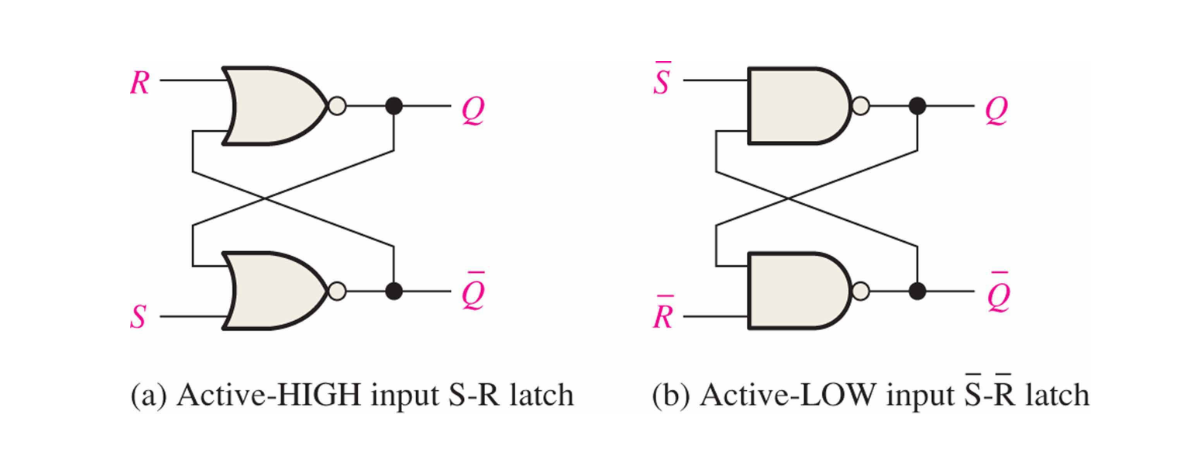
\includegraphics{./assets/SRLatch.png}
\caption{SR Latch}
\end{figure}

\textbf{Two Stable States: (For active-high inputs)}

\begin{enumerate}
\def\labelenumi{\arabic{enumi}.}
\tightlist
\item
  Set State: When \(S=1\) and \(R=0\), the latch is set, and the output
  \(Q\) is 1, while \(\overline{Q}\) is 0.
\item
  Reset State: When \(S=0\) and \(R=1\), the latch is reset, and the
  output \(Q\) is 0, while \(\overline{Q}\) is 1.
\end{enumerate}

\textbf{Indeterminate State:} When \(S=0\) and \(R=0\), both outputs
\(Q\) and \(\overline{Q}\) will remain unchanged.

\textbf{Invalid State:} When \(S=1\) and \(R=1\), both outputs \(Q\) and
\(\overline{Q}\) will be 0, which violates the principle of mutual
exclusivity of the outputs. This state is considered invalid and should
be avoided in practical applications.

\textbf{Truth Table:}

\begin{longtable}[]{@{}llll@{}}
\toprule\noalign{}
\(S\) & \(R\) & \(Q\) (Next State) & \(\overline{Q}\) (Next State) \\
\midrule\noalign{}
\endhead
\bottomrule\noalign{}
\endlastfoot
0 & 0 & Q (No Change) & \(\overline{Q}\) (No Change) \\
0 & 1 & 0 & 1 \\
1 & 0 & 1 & 0 \\
1 & 1 & Invalid & Invalid \\
\end{longtable}

(Truth table for active-low inputs latches:)

\begin{longtable}[]{@{}
  >{\raggedright\arraybackslash}p{(\columnwidth - 6\tabcolsep) * \real{0.0588}}
  >{\raggedright\arraybackslash}p{(\columnwidth - 6\tabcolsep) * \real{0.0588}}
  >{\raggedright\arraybackslash}p{(\columnwidth - 6\tabcolsep) * \real{0.3137}}
  >{\raggedright\arraybackslash}p{(\columnwidth - 6\tabcolsep) * \real{0.5686}}@{}}
\toprule\noalign{}
\begin{minipage}[b]{\linewidth}\raggedright
\(\overline{S}\)
\end{minipage} & \begin{minipage}[b]{\linewidth}\raggedright
\(\overline{R}\)
\end{minipage} & \begin{minipage}[b]{\linewidth}\raggedright
\(Q\) (Next State)
\end{minipage} & \begin{minipage}[b]{\linewidth}\raggedright
\(\overline{Q}\) (Next State)
\end{minipage} \\
\midrule\noalign{}
\endhead
\bottomrule\noalign{}
\endlastfoot
1 & 1 & Q (No Change) & \(\overline{Q}\) (No Change) \\
1 & 0 & 0 & 1 \\
0 & 1 & 1 & 0 \\
0 & 0 & Invalid & Invalid \\
\end{longtable}

The logic symbol of an S-R latch is shown below:

\begin{figure}
\centering
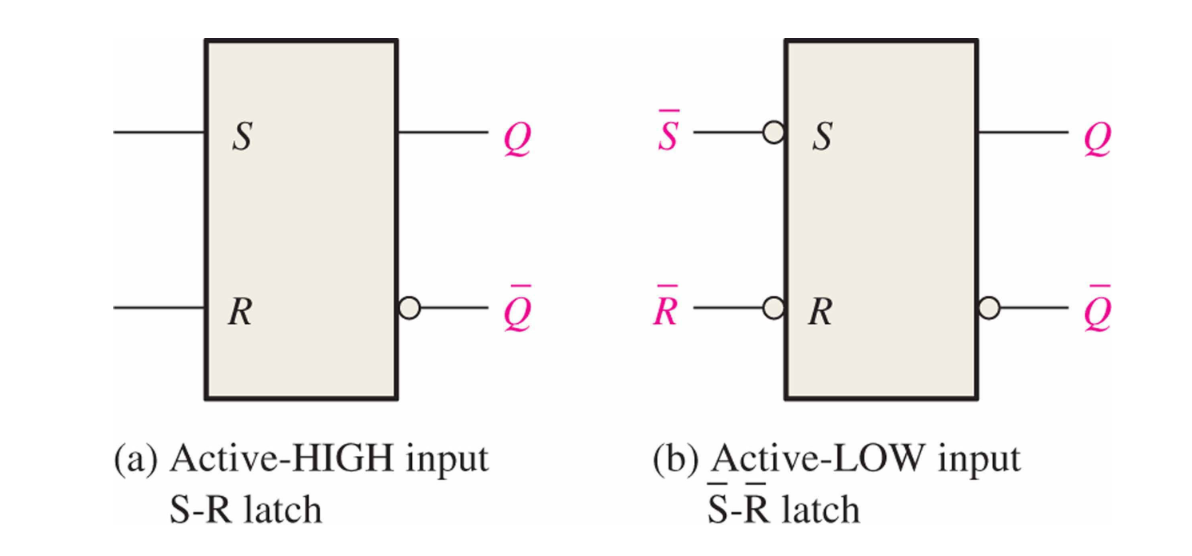
\includegraphics{./assets/SymbolLatch.png}
\caption{SR Latch Symbol}
\end{figure}

\subsubsection{Variation 1: Gated S-R
Latch}\label{variation-1-gated-s-r-latch}

\begin{figure}
\centering
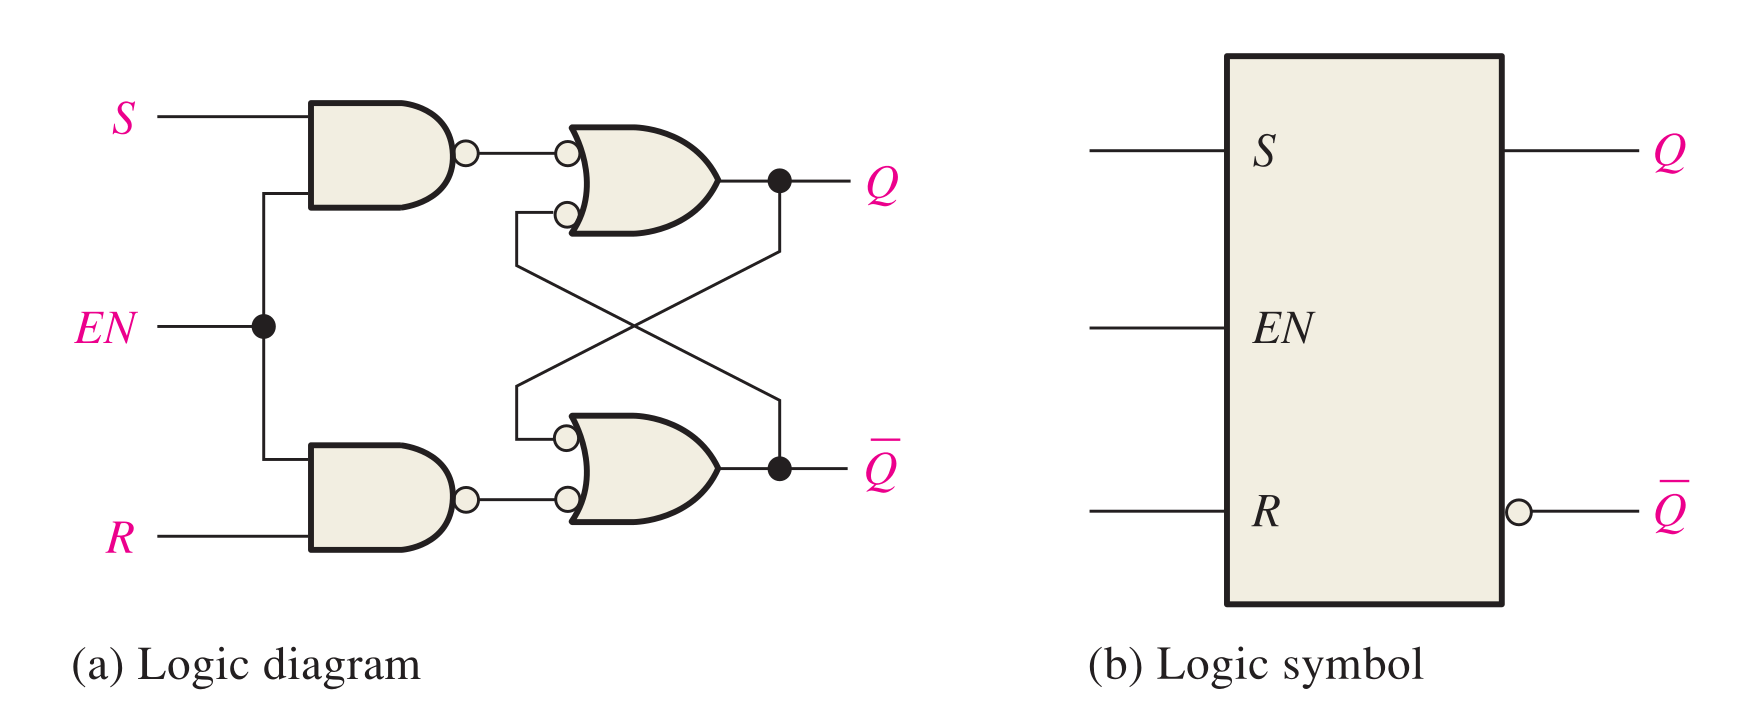
\includegraphics{./assets/GatedSRLatch.png}
\caption{SR Latch with Enable}
\end{figure}

The gated S-R latch is a variation of the basic S-R latch that includes
an enable input (EN). The enable input allows the latch to be
controlled, so that it only responds to the S and R inputs when the
enable signal is active.

Note that the Gated S-R latch shown in the figure above is an
\textbf{active-high} gated S-R latch. The NAND gate at the input side
translate the active-high inputs to active-low inputs for the ordinary
active-low S-R latch.

\textbf{Truth Table:}

\begin{longtable}[]{@{}lllll@{}}
\toprule\noalign{}
EN & S & R & Q (Next State) & \(\overline{Q}\) (Next State) \\
\midrule\noalign{}
\endhead
\bottomrule\noalign{}
\endlastfoot
0 & X & X & Q (No Change) & \(\overline{Q}\) (No Change) \\
1 & 0 & 0 & Q (No Change) & \(\overline{Q}\) (No Change) \\
1 & 0 & 1 & 0 & 1 \\
1 & 1 & 0 & 1 & 0 \\
1 & 1 & 1 & Invalid & Invalid \\
\end{longtable}

\subsubsection{Variation 2: Gated D
Latch}\label{variation-2-gated-d-latch}

To prevent the invalid state of the S-R latch, we can use a D latch,
which has only one input (D) and an enable input (EN). The D latch
ensures that the output is always valid by connecting the D input to
both the S and R inputs of an S-R latch, with one of them inverted.

\begin{figure}
\centering
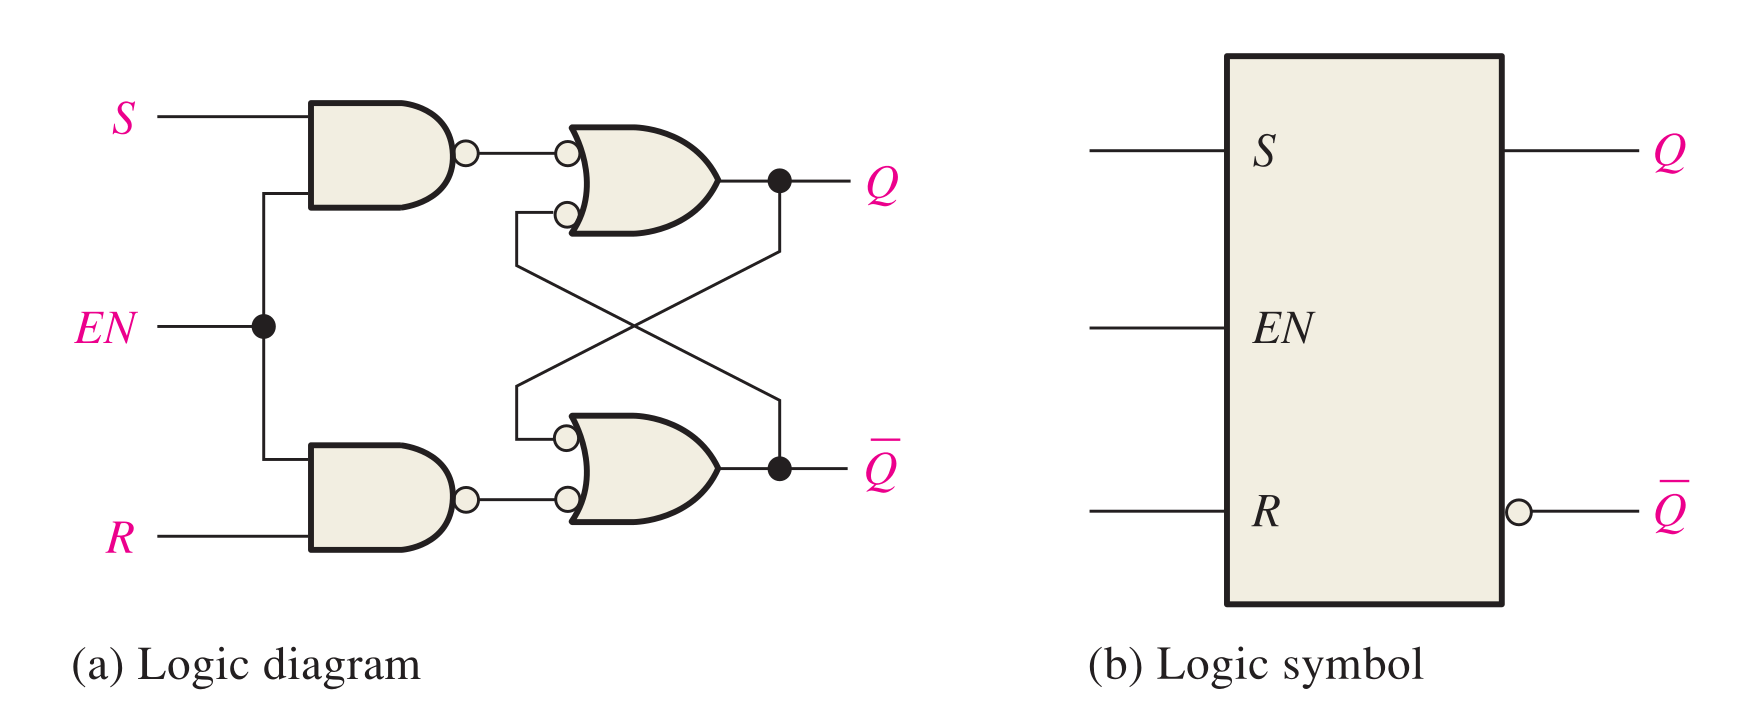
\includegraphics{./assets/DLatch.png}
\caption{D Latch}
\end{figure}

\textbf{Truth Table:}

\begin{longtable}[]{@{}llll@{}}
\toprule\noalign{}
EN & D & Q (Next State) & \(\overline{Q}\) (Next State) \\
\midrule\noalign{}
\endhead
\bottomrule\noalign{}
\endlastfoot
0 & X & Q (No Change) & \(\overline{Q}\) (No Change) \\
1 & 0 & 0 & 1 \\
1 & 1 & 1 & 0 \\
\end{longtable}

\subsection{7.2 Flip-Flops}\label{flip-flops}

A flip-flop is edge-triggered: it samples input only around a clock
transition. Important timing requirements include setup time, hold time,
clock-to-output delay, and maximum clock frequency. Violating setup or
hold time can cause metastability, where the output temporarily fails to
settle to a valid logic level.

\textbf{Flip-flops (FF)} share some structural ideas with latches, but
they are edge-triggered rather than level-triggered. In other words,
flip-flops sample the input data only at specific moments (rising or
falling edge of the clock signal), while latches are transparent and can
change their output as long as the enable signal is active.

\subsubsection{Variation 1: Edge-triggered S-R
FF}\label{variation-1-edge-triggered-s-r-ff}

This kind of variation can be implemented by replacing the enable input
of a gated S-R latch with a clock signal, and adding some logic gates to
ensure that the S and R inputs are only sampled at the rising edge of
the clock signal.

\textbf{Truth Table:}

\begin{longtable}[]{@{}lllll@{}}
\toprule\noalign{}
CLK & S & R & Q (Next State) & \(\overline{Q}\) (Next State) \\
\midrule\noalign{}
\endhead
\bottomrule\noalign{}
\endlastfoot
0 & X & X & Q (No Change) & \(\overline{Q}\) (No Change) \\
1 & 0 & 0 & Q (No Change) & \(\overline{Q}\) (No Change) \\
1 & 0 & 1 & 0 & 1 \\
1 & 1 & 0 & 1 & 0 \\
1 & 1 & 1 & Invalid & Invalid \\
\end{longtable}

\emph{The 1 of the CLK means one edge of the clock signal, which can be
either the rising edge or the falling edge, depending on the design of
the flip-flop.}

The detection of the rising edge can be implemented by the propagation
delay of the logic gates.

\begin{figure}
\centering
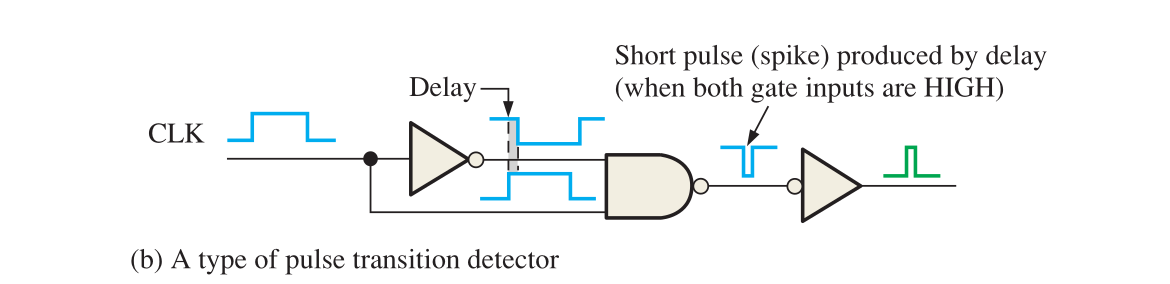
\includegraphics{./assets/edgeTrigger.png}
\caption{Edge-triggered S-R FF}
\end{figure}

\subsubsection{Variation 2: Edge-triggered D
FF}\label{variation-2-edge-triggered-d-ff}

This kind of variation can be implemented by replacing the enable input
of a gated D latch with a clock signal, and adding some logic gates to
ensure that the D input is only sampled at the rising edge of the clock
signal.

\subsubsection{Variation 3: Edge-triggered J-K
FF}\label{variation-3-edge-triggered-j-k-ff}

\begin{figure}
\centering
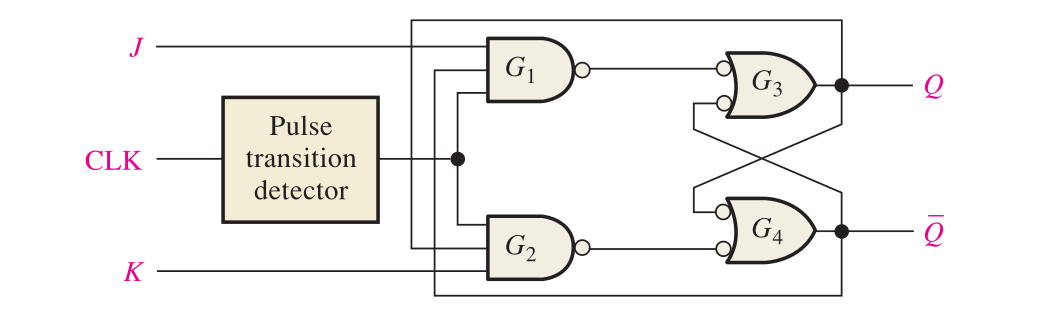
\includegraphics{./assets/JKFF.png}
\caption{Edge-triggered J-K FF}
\end{figure}

The J-K flip-flop is a versatile edge-triggered flip-flop that can be
used to implement various types of sequential logic circuits. It has two
inputs, J and K, and a clock input (CLK). The behavior of the J-K
flip-flop is defined by the following truth table:

\textbf{Truth Table:}

\begin{longtable}[]{@{}lllll@{}}
\toprule\noalign{}
CLK & J & K & Q (Next State) & \(\overline{Q}\) (Next State) \\
\midrule\noalign{}
\endhead
\bottomrule\noalign{}
\endlastfoot
0 & X & X & Q (No Change) & \(\overline{Q}\) (No Change) \\
1 & 0 & 0 & Q (No Change) & \(\overline{Q}\) (No Change) \\
1 & 0 & 1 & 0 & 1 \\
1 & 1 & 0 & 1 & 0 \\
1 & 1 & 1 & \(\overline{Q}\) (Toggle) & \(Q\) (Toggle) \\
\end{longtable}

As you can see, the J-K flip-flop \textbf{does not} have an invalid
state, which makes it more reliable than the S-R FF. When both J and K
are 1, the output toggles, which can be useful in certain applications
such as counters and shift registers.

\subsubsection{Variation 4: Async Reset and Set JK
FF}\label{variation-4-async-reset-and-set-jk-ff}

\begin{figure}
\centering
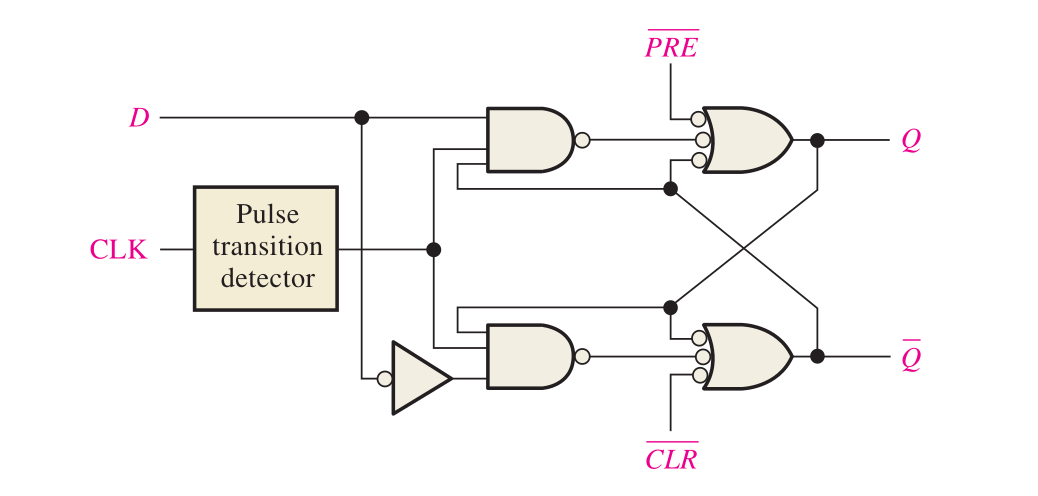
\includegraphics{./assets/asyncJKFF.png}
\caption{Async Reset and Set JK FF}
\end{figure}

The asynchronous reset and set J-K flip-flop is a variation of the
standard J-K flip-flop that includes additional inputs for asynchronous
reset (R) and set (S). These inputs allow the flip-flop to be reset or
set independently of the clock signal, providing more control over the
state of the flip-flop.

Note that the JKFF with asynchronous reset and set shown in the figure
above is an \textbf{active-high} JKFF. But the \textbf{PRE} and
\textbf{CLR} inputs are active-low, which means that they will reset or
set the flip-flop when they are 0.

\subsubsection{Variation 5: Master-Slave JK
FF}\label{variation-5-master-slave-jk-ff}

The master-slave J-K flip-flop is a variation of the standard J-K
flip-flop that consists of two J-K flip-flops connected in series. The
first flip-flop (the master) is triggered by the clock signal, while the
second flip-flop (the slave) is triggered by the output of the master
flip-flop. This configuration allows for edge-triggered operation and
eliminates the possibility of race conditions, making it more reliable
for certain applications.

\subsubsection{Application of J-K FF:
Counters}\label{application-of-j-k-ff-counters}

\begin{figure}
\centering
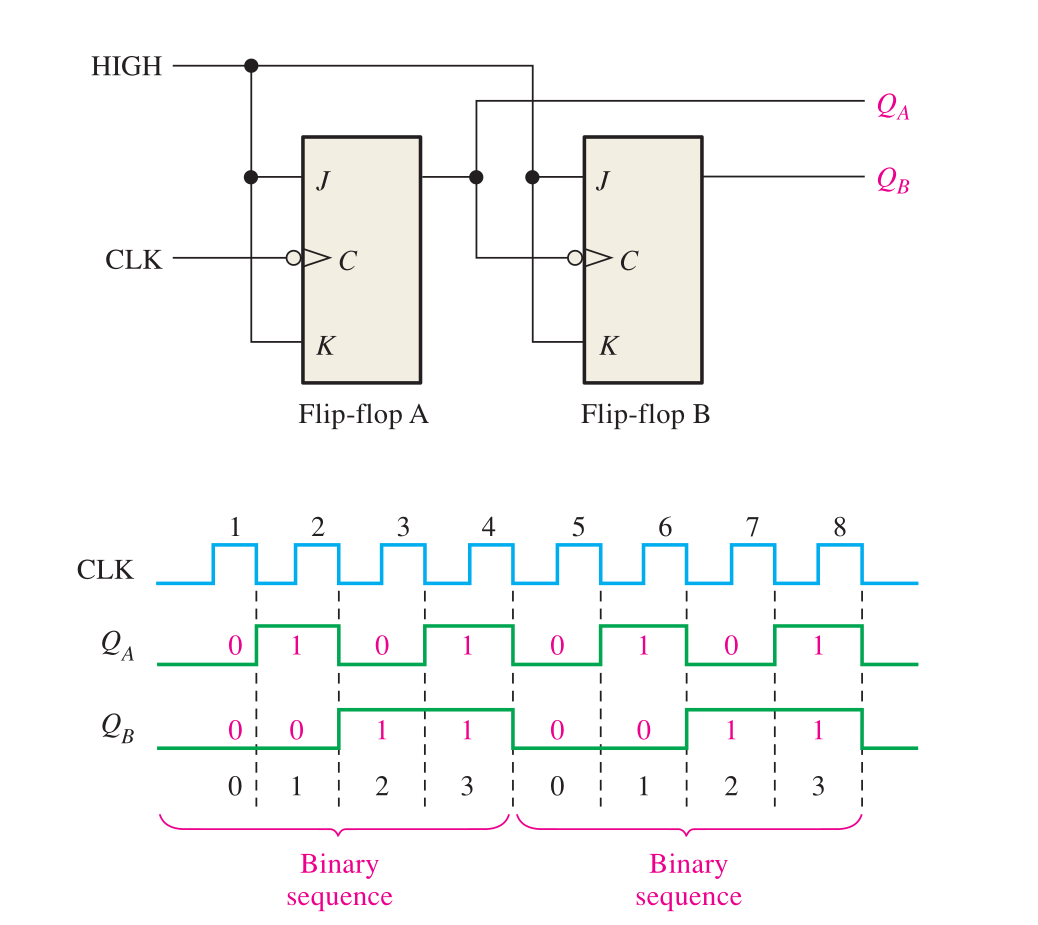
\includegraphics{./assets/Counter.png}
\caption{Counter}
\end{figure}

A counter is a sequential logic circuit that counts the number of clock
pulses. It can be implemented using J-K flip-flops by connecting the
output of one flip-flop to the clock input of the next flip-flop, and
configuring the J and K inputs to toggle the state of each flip-flop on
each clock pulse.

The cascade connection of J-K flip-flops allows for the creation of
binary counters, which can count in binary from 0 to a maximum value
determined by the number of flip-flops used. For example, a 3-bit
counter can count from 0 to 7 (000 to 111 in binary) using three J-K
flip-flops.

\subsubsection{Schmitt Trigger}\label{schmitt-trigger}

A Schmitt trigger is a type of comparator circuit that incorporates
hysteresis to provide noise immunity and a clean output signal. It is
commonly used in digital circuits to convert noisy or slow-changing
input signals into clean, fast transitions.

\begin{itemize}
\tightlist
\item
  Upper Threshold Voltage (\(V_{UT}\)): The voltage level at which the
  output transitions from low to high when the input signal is rising.
\item
  Lower Threshold Voltage (\(V_{LT}\)): The voltage level at which the
  output transitions from high to low when the input signal is falling.
\end{itemize}

Only when the input voltage exceeds the upper threshold voltage
(\(V_{UT}\)) will the output switch to high, and only when the input
voltage falls below the lower threshold voltage (\(V_{LT}\)) will the
output switch to low. This hysteresis effect helps to prevent false
triggering due to noise or slow input transitions.

\subsection{7.3 One-Shots (Monostable
Multivibrators)}\label{one-shots-monostable-multivibrators}

\begin{figure}
\centering
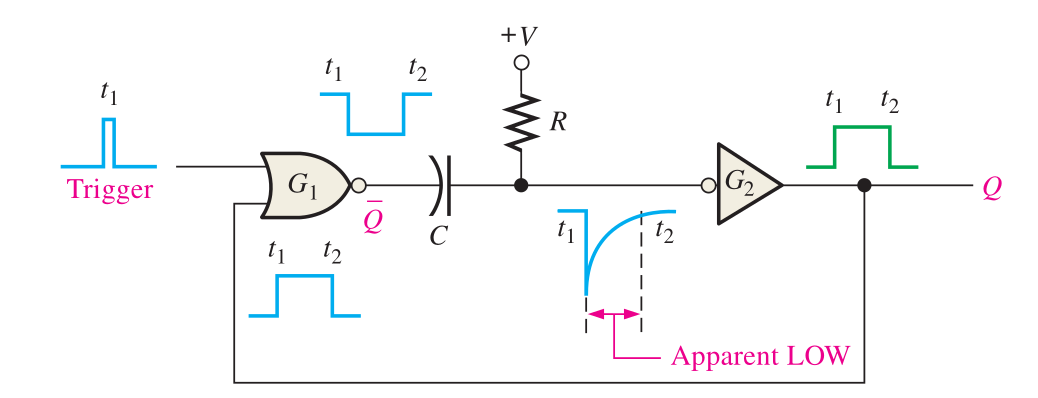
\includegraphics{./assets/simpleoneshot.png}
\caption{One-Shot}
\end{figure}

A one-shot, also known as a monostable multivibrator, is a type of
sequential logic circuit that generates a single output pulse of a
specified duration in response to an input trigger signal. The output
pulse is generated only once for each trigger event, and the circuit
returns to its stable state after the pulse is generated.

\textbf{Non-retriggerable One-Shot:}

\begin{itemize}
\tightlist
\item
  Once triggered, the one-shot will generate a pulse of fixed duration
  regardless of any additional trigger signals that may occur during the
  pulse duration. The one-shot will not respond to any new trigger
  signals until it has completed its current pulse and returned to its
  stable state.
\end{itemize}

\begin{figure}
\centering
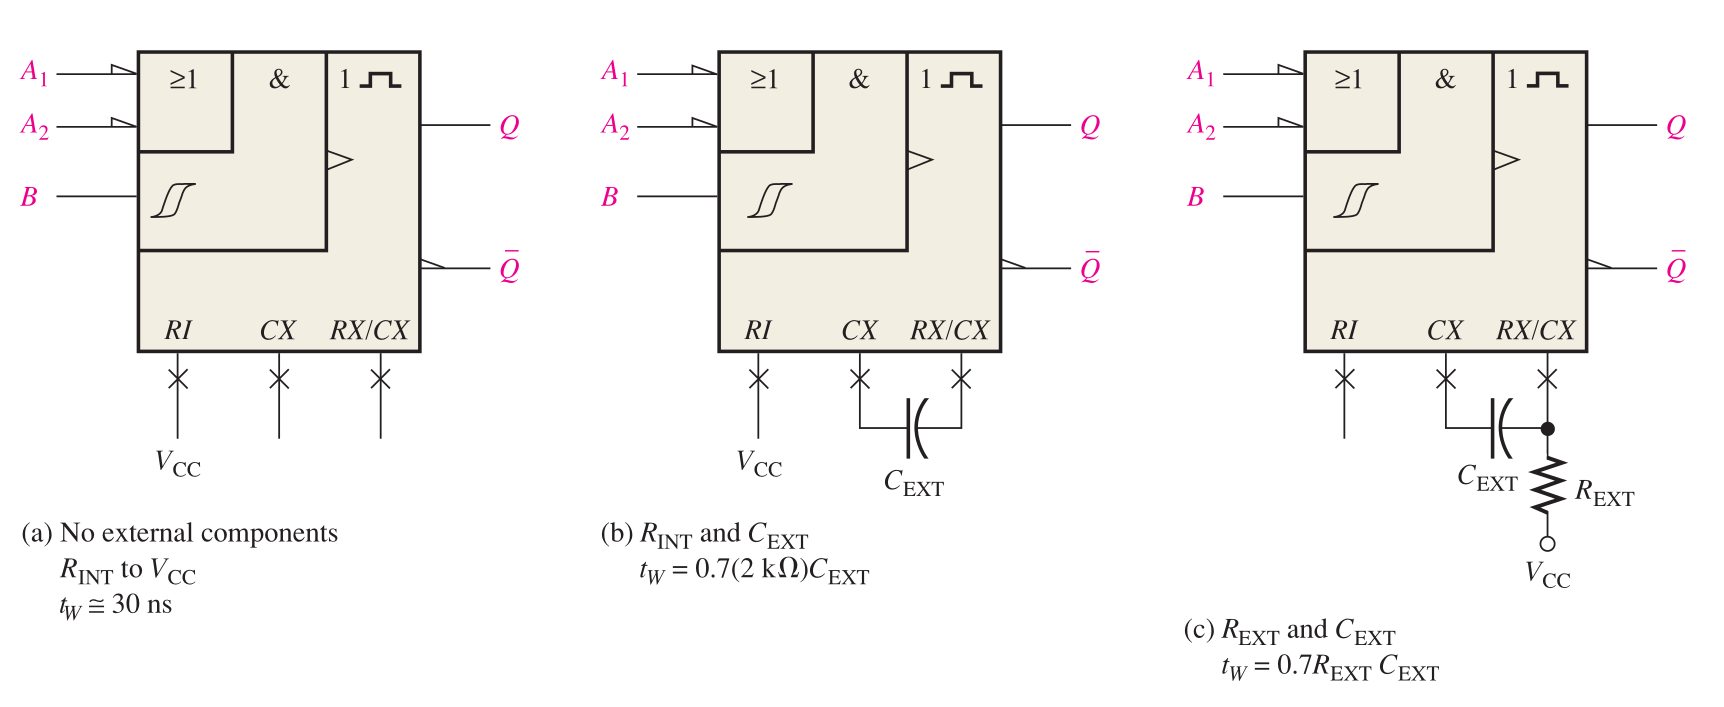
\includegraphics{./assets/usageoneshot.png}
\caption{Usage of One-Shot}
\end{figure}

\[
t_w = RC \ln\left(\frac{V_{CC}}{V_{CC} - V_{TH}}\right) \approx 0.693 RC \approx 0.7 RC
\]

When \(R\) is expressed in \(\mathrm{k\Omega}\) and \(C\) in
\(\mathrm{pF}\), \(t_w\) is obtained in \(\mathrm{ns}\).

\subsection{7.4 555 Timer}\label{timer}

The 555 timer combines analog threshold detection with digital switching
behavior. Internally it uses comparators, a latch, a discharge
transistor, and a resistor divider, which makes it a useful bridge
between analog timing networks and digital pulses.

\begin{figure}
\centering
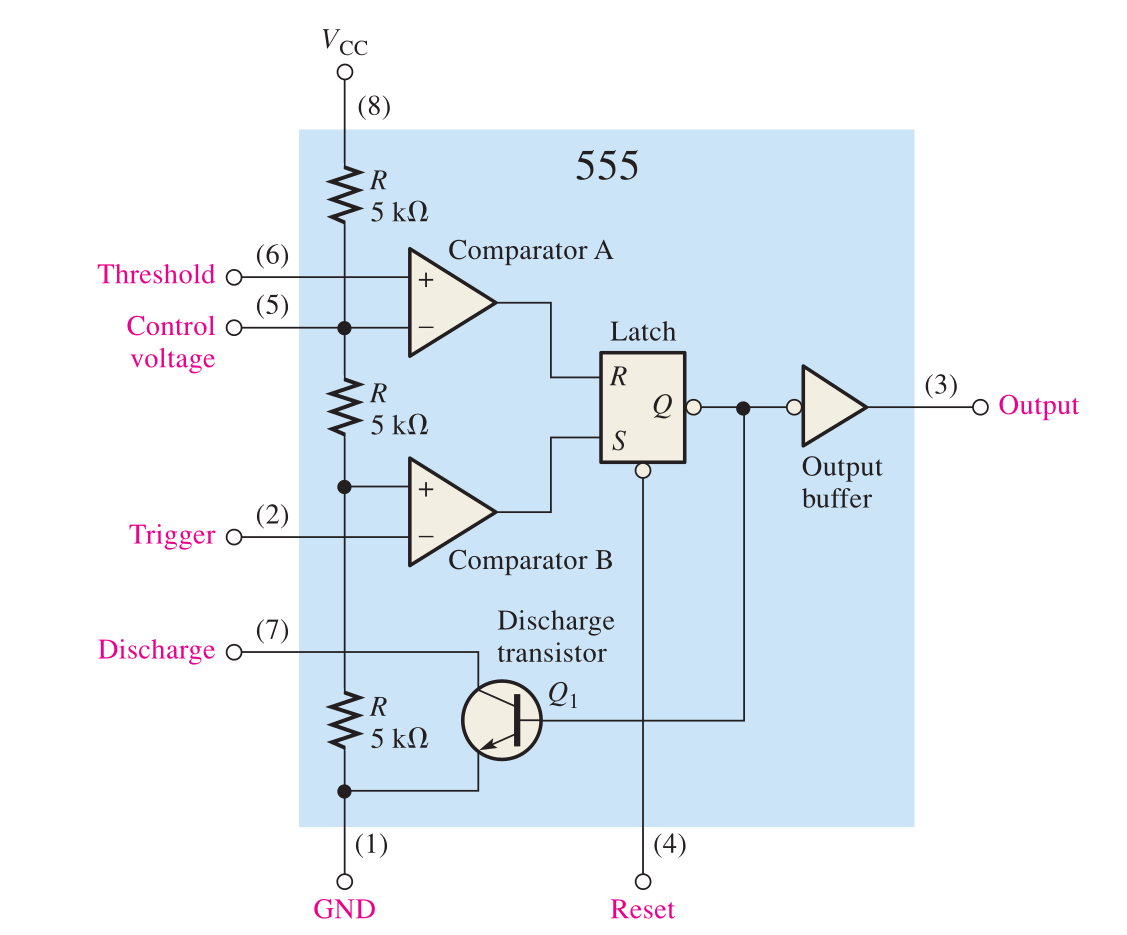
\includegraphics{./assets/555timer.png}
\caption{555 Timer}
\end{figure}

The 555 timer is a versatile integrated circuit that can be used in
various applications, including timers, pulse generators, and
oscillators. It can operate in three different modes: monostable mode,
astable mode, and bistable mode.

\textbf{Monostable Mode:} In monostable mode, the 555 timer functions as
a one-shot pulse generator. When triggered by an input signal, it
produces a single output pulse of a specified duration determined by an
external resistor and capacitor.

\begin{figure}
\centering
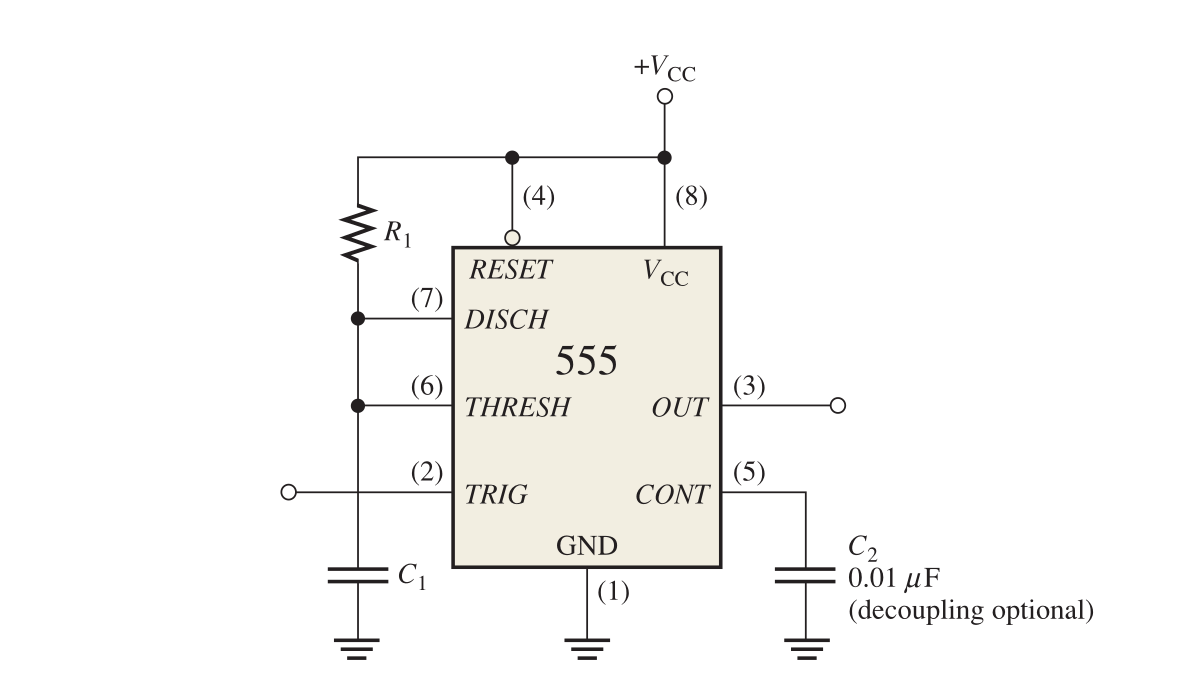
\includegraphics{./assets/555timeroneshot.png}
\caption{555 Timer Monostable Mode}
\end{figure}

\[t_w = 1.1 R_1C_1\]

The principle is shown in the figure below:

\begin{figure}
\centering
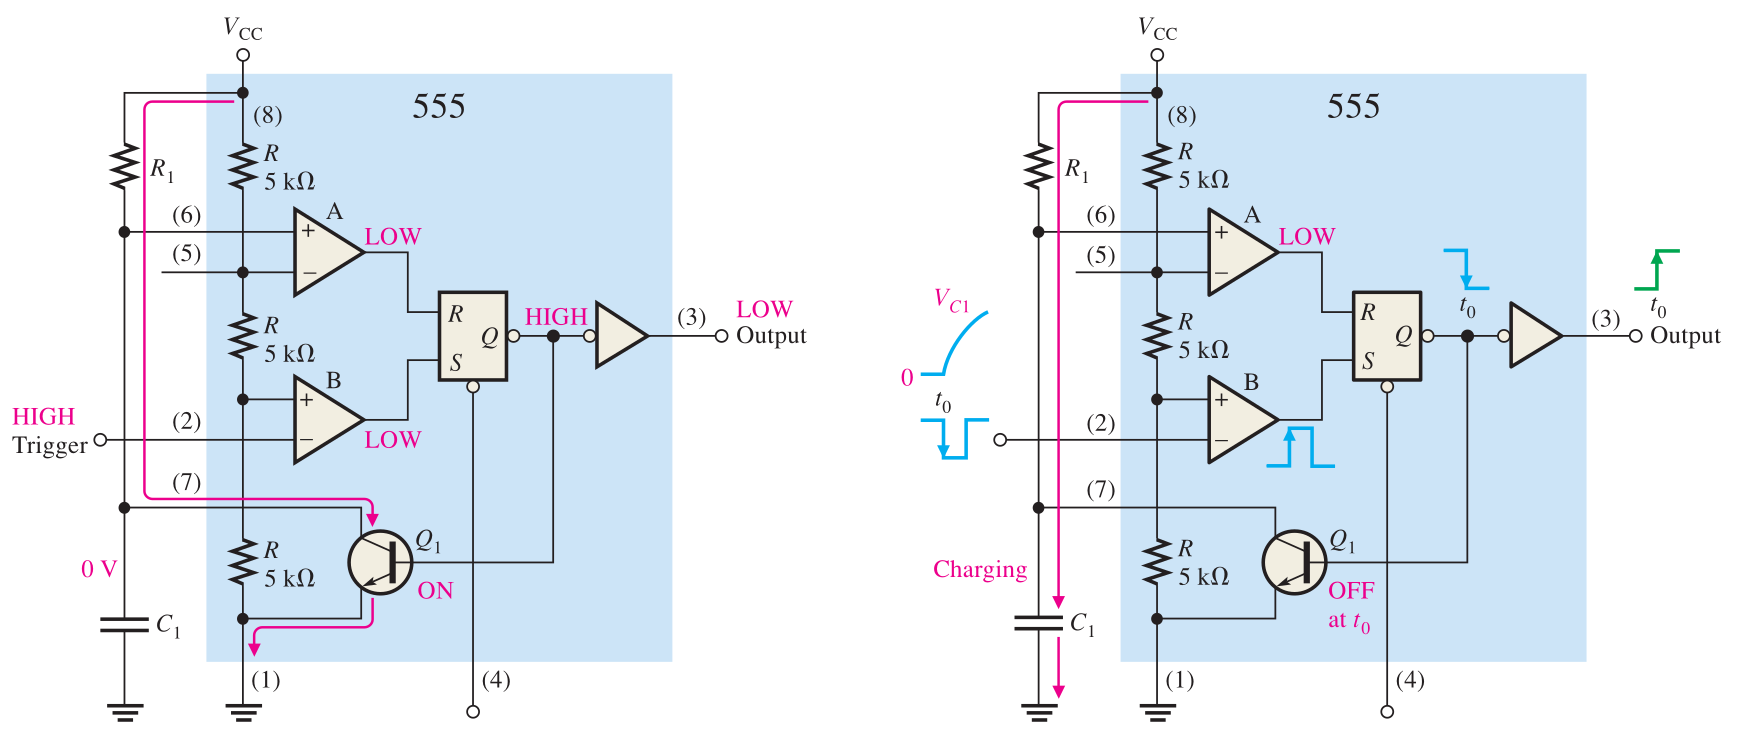
\includegraphics{./assets/principle.png}
\caption{Monostable Mode Principle}
\end{figure}

\textbf{Astable Multivibrators:}

In astable mode, the 555 timer functions as an oscillator, generating a
continuous square wave output without the need for an external trigger.
The frequency and duty cycle of the output waveform can be adjusted
using external resistors and capacitors.

In such scenario, the 555 timer should be connected as shown in the
figure below:

\begin{figure}
\centering
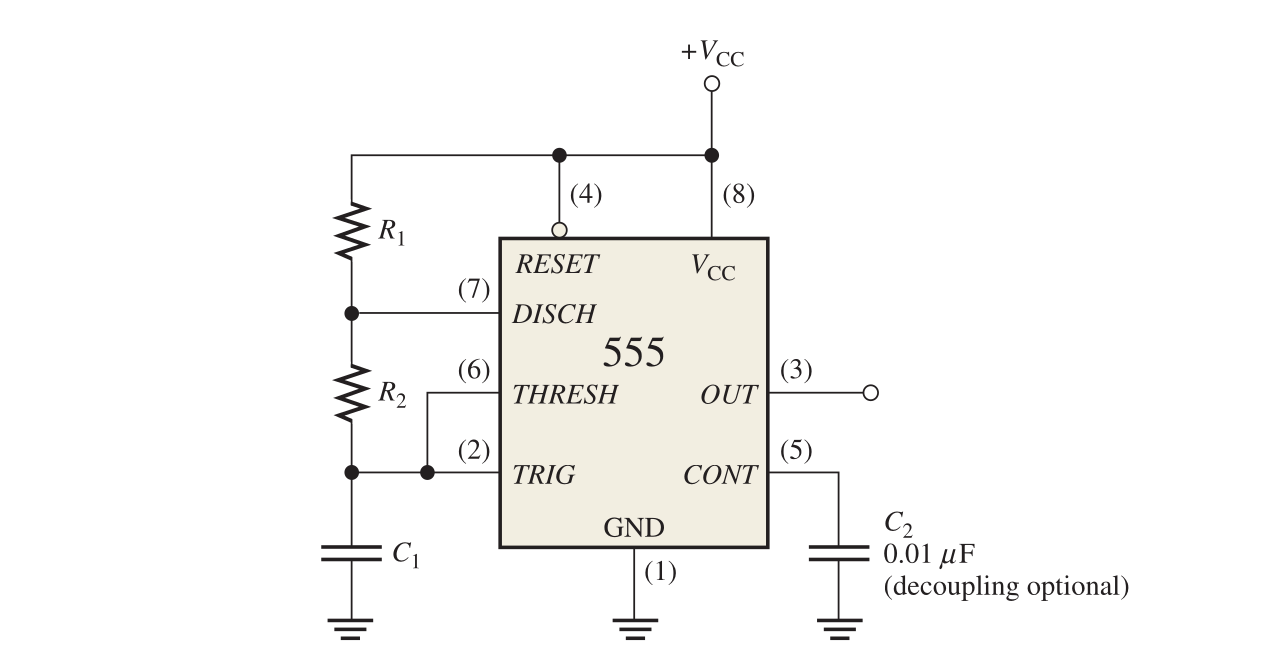
\includegraphics{./assets/timerconnection.png}
\caption{555 Timer Astable Mode}
\end{figure}

\begin{figure}
\centering
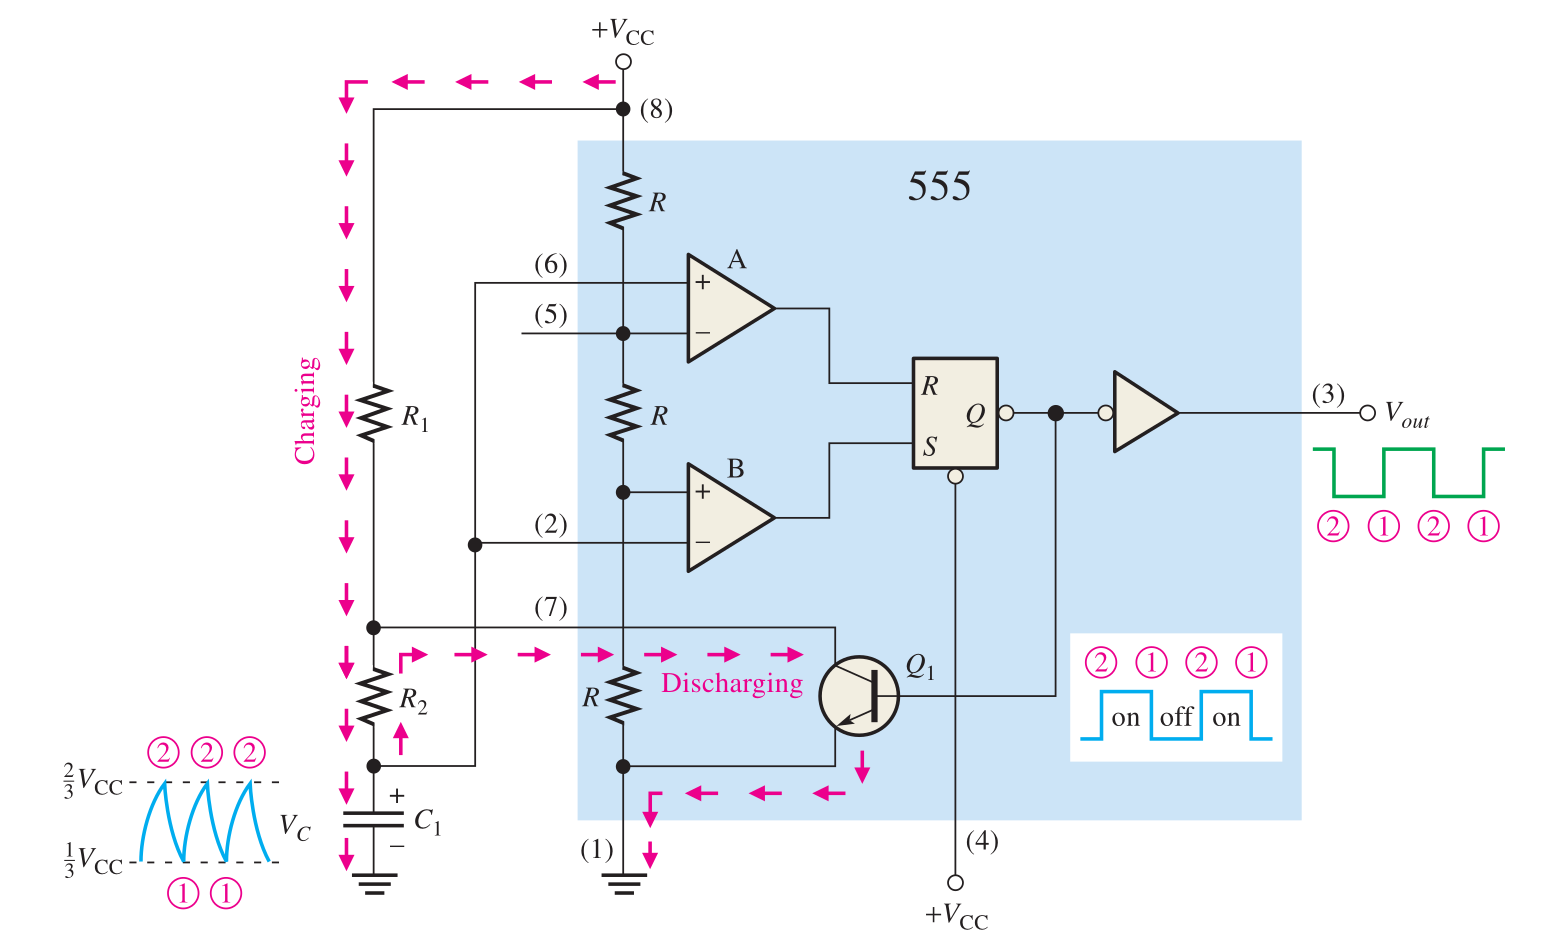
\includegraphics{./assets/timeroperation.png}
\caption{555 Timer Astable Mode}
\end{figure}

\[f = \frac{1.44}{(R_1 + 2R_2)C_1}\]

\[t_H = 0.7(R_1 + R_2)C_1, \quad t_L = 0.7 R_2 C_1\]

\[\text{Duty Cycle} = \frac{t_H}{t_H + t_L} = \frac{R_1 + R_2}{R_1 + 2R_2}\]

\begin{notebox}{Review after Chapter 7}
Check that you can distinguish latches from flip-flops, explain the invalid state of an S-R latch, describe J-K toggle behavior, and calculate basic 555 timer pulse widths or astable frequency.
\end{notebox}

\section{Chapter 9*: Counters}\label{chapter-9-counters}

\begin{chapterbox}{Chapter focus}
Counters are sequential circuits that move through a defined state sequence. The central design question is not only what number comes next, but also how the flip-flop inputs must be driven to force that next state.
\end{chapterbox}

\emph{Chapter 8 is outside the scope of this summary}

In previous chapters, we have already introduced the concept of counters
and how to implement them using J-K flip-flops. In this chapter, we will
explore different types of counters and their applications in more
detail.

With respect to the previous content, we can classify counters into two
categories: \textbf{Asynchronous Counters} and \textbf{Synchronous
Counters}.

The counters we introduced in the previous chapter are asynchronous
counters, also known as ripple counters. In an asynchronous counter, the
flip-flops are not clocked simultaneously. The output of one flip-flop
serves as the clock input for the next flip-flop in the sequence. This
means that the counting operation ripples through the flip-flops, which
can lead to propagation delays and limit the maximum counting speed.

\subsection{Synchronous Counters}\label{synchronous-counters}

\begin{figure}
\centering
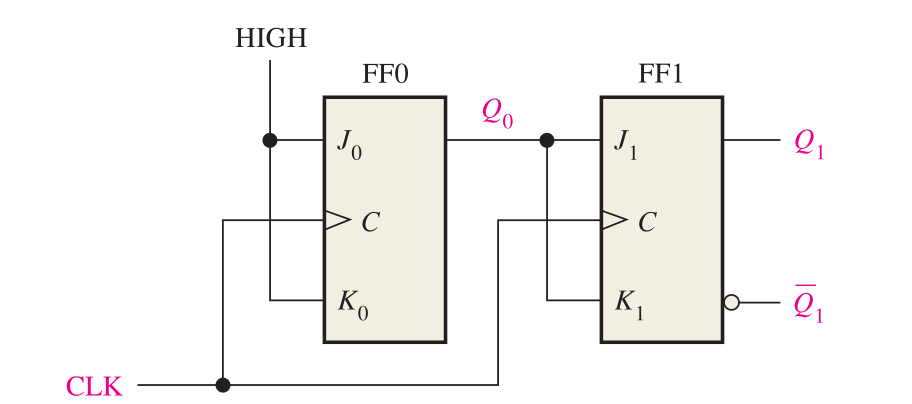
\includegraphics{./assets/synccounter.png}
\caption{2-bit Synchronous Counter}
\end{figure}

In a synchronous counter, all the flip-flops are clocked simultaneously
by a common clock signal. This means that all the flip-flops change
their state at the same time, which eliminates the propagation delay
issue present in asynchronous counters and allows for higher counting
speeds.

Note that the design of synchronous counters is to make controlled use
of the propagation delay of the logic gates. In this case the small
delay through the gating logic is part of the timing design rather than
only a limitation, which allows the counter to operate correctly at
higher frequencies.

The figure below shows the design of a 4-bit synchronous counter:

\begin{figure}
\centering
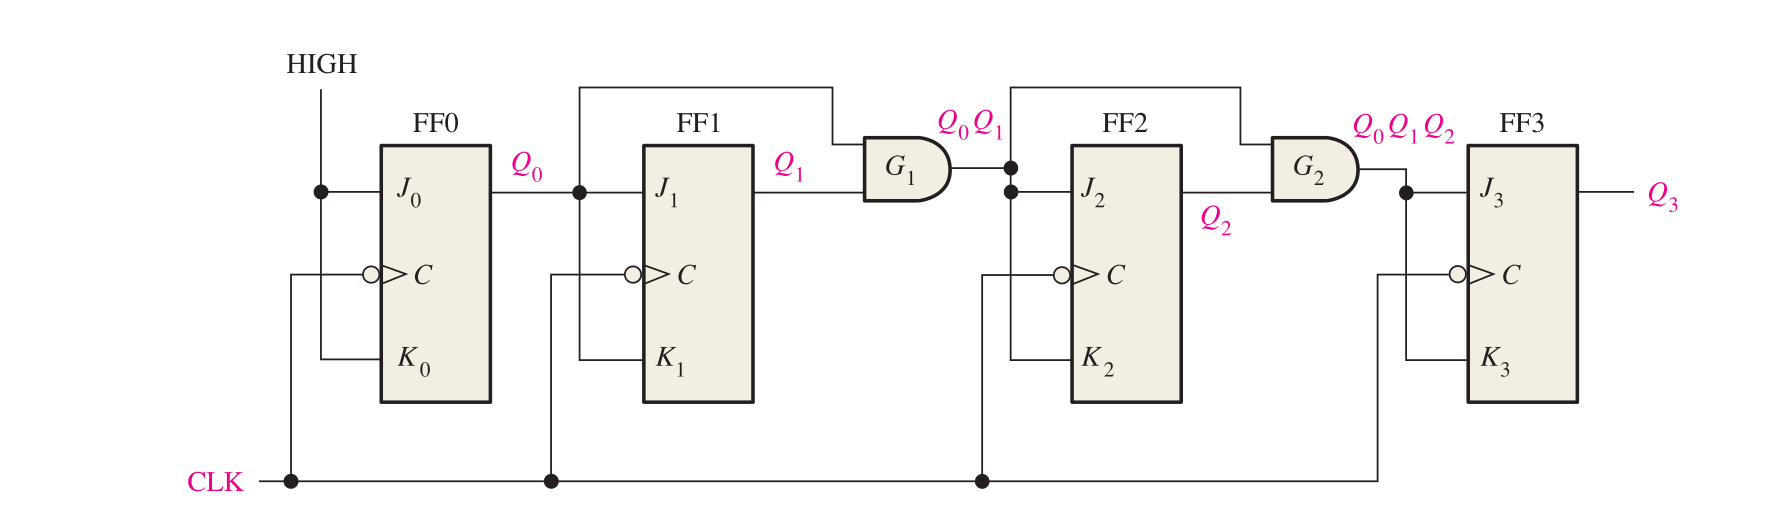
\includegraphics{./assets/4bitsync.png}
\caption{4-bit Synchronous Counter}
\end{figure}

\[
\begin{aligned}
J_0 &= 1, & J_1 &= Q_0, & J_2 &= Q_0 \cdot Q_1,\\
J_3 &= Q_0 \cdot Q_1 \cdot Q_2, & J_n &= Q_0 \cdot Q_1 \cdots Q_{n-1}.
\end{aligned}
\]

\textbf{74HC163}

\emph{Function Table:}

\begin{center}
\small
\begin{tabular}{lcccccccc}
\toprule
Operating Mode & $\overline{CLR}$ & CLK & ENP & ENT & $\overline{LOAD}$ & D & Q & RCO \\
\midrule
Reset   & 0 & 1 & X & X & X & X & 0   & 0 \\
Load    & 1 & 1 & X & X & 0 & D & D   & 0 \\
Count   & 1 & 1 & 1 & 1 & 1 & X & Q+1 & RCO \\
Inhibit & 1 & X & 0 & X & 1 & X & Q   & RCO \\
Inhibit & 1 & X & X & 0 & 1 & X & Q   & 0 \\
\bottomrule
\end{tabular}
\end{center}

\begin{itemize}
\tightlist
\item
  \(\overline{CLR}\): Active-low asynchronous clear input. When this
  input is low, the counter is reset to 0 regardless of the clock or
  other inputs.
\item
  \(CLK\): Clock input. The counter increments on the rising edge of the
  clock signal when counting is enabled.
\item
  \(ENP\): Count enable parallel input. This input must be high for the
  counter to increment on the clock edge.
\item
  \(ENT\): Count enable toggle input. This input must be high for the
  counter to increment on the clock edge.
\item
  \(\overline{LOAD}\): Active-low load input. When this input is low,
\item
  \(D\): Data inputs. These inputs are used to load a specific value
  into the counter when the load input is activated.
\end{itemize}

\textbf{Note that the ENP and ENT inputs are used together to enable
counting. Both inputs must be high for the counter to increment on the
clock edge. If either input is low, the counter will not increment and
will maintain its current state.}

\textbf{74LS190}: Synchronous Up/Down Decade Counter

The \(D/\overline{U}\) input determines the counting direction. When
\(D/\overline{U}\) is high, the counter counts down; when
\(D/\overline{U}\) is low, the counter counts up.

\subsection{Design a Counter}\label{design-a-counter}

For custom counters, unused states should not be ignored. A robust
design either sends unused states back into the legal sequence or
ensures that they cannot be entered during normal operation.

To design a counter, we need to follow these steps:

\begin{itemize}
\tightlist
\item
  Determine the state diagram.
\item
  Derive a next state table from the state diagram.
\item
  Derive the flip-flop input equations from the next state table.
\item
  Implement the flip-flop input equations using Karnaugh maps or Boolean
  algebra to simplify the logic.
\end{itemize}

\textbf{Characteristics Equation of J-K FF:}
\[Q_{\text{next}} = J \cdot \overline{Q} + \overline{K} \cdot Q\]

\emph{Function Table of J-K FF:}

\begin{center}
\small
\begin{tabular}{cccc}
\toprule
$Q_N$ & $Q_{N+1}$ & $J$ & $K$ \\
\midrule
0 & 0 & 0 & X \\
0 & 1 & 1 & X \\
1 & 0 & X & 1 \\
1 & 1 & X & 0 \\
\bottomrule
\end{tabular}
\end{center}

So using this function table, we can derive the flip-flop input
equations for each flip-flop in the counter design. Then we can simplify
these equations using Karnaugh maps or Boolean algebra to get the final
implementation of the counter.

Here is an example of designing a 3-bit synchronous counter that counts
from 0 to 7:

\begin{itemize}
\tightlist
\item
  State Diagram:
\end{itemize}

\[
000 \rightarrow 001 \rightarrow 010 \rightarrow 011 \rightarrow 100 \rightarrow 101 \rightarrow 110 \rightarrow 111 \rightarrow 000
\]

\begin{itemize}
\tightlist
\item
  Next State Table:
\end{itemize}

\begin{longtable}[]{@{}ll@{}}
\toprule\noalign{}
Current State (Q2 Q1 Q0) & Next State (Q2' Q1' Q0') \\
\midrule\noalign{}
\endhead
\bottomrule\noalign{}
\endlastfoot
000 & 001 \\
001 & 010 \\
010 & 011 \\
011 & 100 \\
100 & 101 \\
101 & 110 \\
110 & 111 \\
111 & 000 \\
\end{longtable}

\begin{itemize}
\tightlist
\item
  Flip-Flop Input Equations:
\end{itemize}

\begin{longtable}[]{@{}llllllll@{}}
\toprule\noalign{}
Q2 Q1 Q0 & Q2' Q1' Q0' & J2 & K2 & J1 & K1 & J0 & K0 \\
\midrule\noalign{}
\endhead
\bottomrule\noalign{}
\endlastfoot
000 & 001 & 0 & X & 0 & X & 1 & X \\
001 & 010 & 0 & X & 1 & X & X & 1 \\
010 & 011 & 0 & X & X & 0 & 1 & X \\
011 & 100 & 1 & X & X & 1 & X & 1 \\
100 & 101 & X & 0 & 0 & X & 1 & X \\
101 & 110 & X & 0 & 1 & X & X & 1 \\
110 & 111 & X & 0 & X & 0 & 1 & X \\
111 & 000 & X & 1 & X & 1 & X & 1 \\
\end{longtable}

\begin{itemize}
\tightlist
\item
  Simplified Flip-Flop Input Equations:
\end{itemize}

\[J_0 = 1, \quad K_0 = 1\]

\[J_1 = Q_0, \quad K_1 = Q_0\]

\[J_2 = Q_1 \cdot Q_0, \quad K_2 = Q_1 \cdot Q_0\]

You can also simplify the equations using Karnaugh maps to get the same
result. The final implementation of the counter can be done using J-K
flip-flops and the derived input equations.

This is the overall process of designing a synchronous counter. The same
steps can be applied to design counters with different counting
sequences, such as up/down counters, decade counters, or custom sequence
counters.

\subsection{Counter Cascading}\label{counter-cascading}

When counters are cascaded, timing must be checked carefully.
Synchronous cascading normally uses terminal-count or ripple-carry
outputs as enable signals while keeping a common clock, which avoids
accumulating ripple delay through multiple stages.

The key to cascading counters is to connect the output of one counter to
the clock input of the next counter. You need to connect the clock to
the CLK of both counters, and connect the \textbf{RCO/TC output of the
first counter to the CTEN or ENP/ENT of the second counter}. This way,
the second counter will increment its count only when the first counter
reaches its maximum count and generates a carry-out signal.

\section{Final Review Checklist}\label{final-review-checklist}

\begin{enumerate}
\def\labelenumi{\arabic{enumi}.}
\tightlist
\item
  Confirm the meaning of each bit pattern before doing arithmetic.
\item
  Check whether a signal is active-high or active-low before reading a
  truth table.
\item
  For combinational circuits, verify the truth table after
  simplification.
\item
  For sequential circuits, check setup time, hold time, propagation
  delay, and unused states.
\item
  For counters, decide whether the design is asynchronous or synchronous
  before analyzing timing.
\end{enumerate}

\section{Image Attribution}\label{image-attribution}

Some figures in this note are taken or adapted from the book
\emph{Digital Fundamentals} by Thomas Floyd. They are included here for
educational study-note purposes; all rights remain with the original
author and publisher.

\end{document}
